\documentclass[twoside]{book}

% Packages required by doxygen
\usepackage{fixltx2e}
\usepackage{calc}
\usepackage{doxygen}
\usepackage[export]{adjustbox} % also loads graphicx
\usepackage{graphicx}
\usepackage[utf8]{inputenc}
\usepackage{makeidx}
\usepackage{multicol}
\usepackage{multirow}
\PassOptionsToPackage{warn}{textcomp}
\usepackage{textcomp}
\usepackage[nointegrals]{wasysym}
\usepackage[table]{xcolor}

% Font selection
\usepackage[T1]{fontenc}
\usepackage[scaled=.90]{helvet}
\usepackage{courier}
\usepackage{amssymb}
\usepackage{sectsty}
\renewcommand{\familydefault}{\sfdefault}
\allsectionsfont{%
  \fontseries{bc}\selectfont%
  \color{darkgray}%
}
\renewcommand{\DoxyLabelFont}{%
  \fontseries{bc}\selectfont%
  \color{darkgray}%
}
\newcommand{\+}{\discretionary{\mbox{\scriptsize$\hookleftarrow$}}{}{}}

% Page & text layout
\usepackage{geometry}
\geometry{%
  a4paper,%
  top=2.5cm,%
  bottom=2.5cm,%
  left=2.5cm,%
  right=2.5cm%
}
\tolerance=750
\hfuzz=15pt
\hbadness=750
\setlength{\emergencystretch}{15pt}
\setlength{\parindent}{0cm}
\setlength{\parskip}{3ex plus 2ex minus 2ex}
\makeatletter
\renewcommand{\paragraph}{%
  \@startsection{paragraph}{4}{0ex}{-1.0ex}{1.0ex}{%
    \normalfont\normalsize\bfseries\SS@parafont%
  }%
}
\renewcommand{\subparagraph}{%
  \@startsection{subparagraph}{5}{0ex}{-1.0ex}{1.0ex}{%
    \normalfont\normalsize\bfseries\SS@subparafont%
  }%
}
\makeatother

% Headers & footers
\usepackage{fancyhdr}
\pagestyle{fancyplain}
\fancyhead[LE]{\fancyplain{}{\bfseries\thepage}}
\fancyhead[CE]{\fancyplain{}{}}
\fancyhead[RE]{\fancyplain{}{\bfseries\leftmark}}
\fancyhead[LO]{\fancyplain{}{\bfseries\rightmark}}
\fancyhead[CO]{\fancyplain{}{}}
\fancyhead[RO]{\fancyplain{}{\bfseries\thepage}}
\fancyfoot[LE]{\fancyplain{}{}}
\fancyfoot[CE]{\fancyplain{}{}}
\fancyfoot[RE]{\fancyplain{}{\bfseries\scriptsize Generated by Doxygen }}
\fancyfoot[LO]{\fancyplain{}{\bfseries\scriptsize Generated by Doxygen }}
\fancyfoot[CO]{\fancyplain{}{}}
\fancyfoot[RO]{\fancyplain{}{}}
\renewcommand{\footrulewidth}{0.4pt}
\renewcommand{\chaptermark}[1]{%
  \markboth{#1}{}%
}
\renewcommand{\sectionmark}[1]{%
  \markright{\thesection\ #1}%
}

% Indices & bibliography
\usepackage{natbib}
\usepackage[titles]{tocloft}
\setcounter{tocdepth}{3}
\setcounter{secnumdepth}{5}
\makeindex

% Hyperlinks (required, but should be loaded last)
\usepackage{ifpdf}
\ifpdf
  \usepackage[pdftex,pagebackref=true]{hyperref}
\else
  \usepackage[ps2pdf,pagebackref=true]{hyperref}
\fi
\hypersetup{%
  colorlinks=true,%
  linkcolor=blue,%
  citecolor=blue,%
  unicode%
}

% Custom commands
\newcommand{\clearemptydoublepage}{%
  \newpage{\pagestyle{empty}\cleardoublepage}%
}

\usepackage{caption}
\captionsetup{labelsep=space,justification=centering,font={bf},singlelinecheck=off,skip=4pt,position=top}

%===== C O N T E N T S =====

\begin{document}

% Titlepage & ToC
\hypersetup{pageanchor=false,
             bookmarksnumbered=true,
             pdfencoding=unicode
            }
\pagenumbering{alph}
\begin{titlepage}
\vspace*{7cm}
\begin{center}%
{\Large D\+AA A1 Convex Hull Algorithms }\\
\vspace*{1cm}
{\large Generated by Doxygen 1.8.13}\\
\end{center}
\end{titlepage}
\clearemptydoublepage
\pagenumbering{roman}
\tableofcontents
\clearemptydoublepage
\pagenumbering{arabic}
\hypersetup{pageanchor=true}

%--- Begin generated contents ---
\chapter{D\+A\+A-\/\+A1}
\label{md_README}
\Hypertarget{md_README}
Convex Hull Algorithms

Run using g++ \hyperlink{base_8cpp}{base.\+cpp} \hyperlink{GeomOps_8cpp}{Geom\+Ops.\+cpp} \hyperlink{VectorOps_8cpp}{Vector\+Ops.\+cpp} \hyperlink{Point_8cpp}{Point.\+cpp} 
\chapter{Namespace Index}
\section{Namespace List}
Here is a list of all namespaces with brief descriptions\+:\begin{DoxyCompactList}
\item\contentsline{section}{\hyperlink{namespaceplotJM}{plot\+JM} }{\pageref{namespaceplotJM}}{}
\item\contentsline{section}{\hyperlink{namespaceplotKPS}{plot\+K\+PS} }{\pageref{namespaceplotKPS}}{}
\end{DoxyCompactList}

\chapter{Class Index}
\section{Class List}
Here are the classes, structs, unions and interfaces with brief descriptions\+:\begin{DoxyCompactList}
\item\contentsline{section}{\hyperlink{classGeomOps}{Geom\+Ops} }{\pageref{classGeomOps}}{}
\item\contentsline{section}{\hyperlink{classPoint}{Point} \\*This defines a 2-\/D point with common functionalities to set and retrieve coordinate values }{\pageref{classPoint}}{}
\item\contentsline{section}{\hyperlink{classStack}{Stack$<$ T $>$} \\*Simple \hyperlink{classStack}{Stack} implementation }{\pageref{classStack}}{}
\item\contentsline{section}{\hyperlink{classVectorOps}{Vector\+Ops} }{\pageref{classVectorOps}}{}
\end{DoxyCompactList}

\chapter{File Index}
\section{File List}
Here is a list of all files with brief descriptions\+:\begin{DoxyCompactList}
\item\contentsline{section}{\hyperlink{base_8cpp}{base.\+cpp} }{\pageref{base_8cpp}}{}
\item\contentsline{section}{\hyperlink{GeomOps_8cpp}{Geom\+Ops.\+cpp} }{\pageref{GeomOps_8cpp}}{}
\item\contentsline{section}{\hyperlink{GeomOps_8h}{Geom\+Ops.\+h} }{\pageref{GeomOps_8h}}{}
\item\contentsline{section}{\hyperlink{plotJM_8py}{plot\+J\+M.\+py} }{\pageref{plotJM_8py}}{}
\item\contentsline{section}{\hyperlink{plotKPS_8py}{plot\+K\+P\+S.\+py} }{\pageref{plotKPS_8py}}{}
\item\contentsline{section}{\hyperlink{Point_8cpp}{Point.\+cpp} }{\pageref{Point_8cpp}}{}
\item\contentsline{section}{\hyperlink{Point_8h}{Point.\+h} }{\pageref{Point_8h}}{}
\item\contentsline{section}{\hyperlink{Stack_8h}{Stack.\+h} }{\pageref{Stack_8h}}{}
\item\contentsline{section}{\hyperlink{VectorOps_8cpp}{Vector\+Ops.\+cpp} }{\pageref{VectorOps_8cpp}}{}
\item\contentsline{section}{\hyperlink{VectorOps_8h}{Vector\+Ops.\+h} }{\pageref{VectorOps_8h}}{}
\end{DoxyCompactList}

\chapter{Namespace Documentation}
\hypertarget{namespaceplotJM}{}\section{plot\+JM Namespace Reference}
\label{namespaceplotJM}\index{plot\+JM@{plot\+JM}}
\subsection*{Variables}
\begin{DoxyCompactItemize}
\item 
int \hyperlink{namespaceplotJM_aa893f2c8f47574915a4cc130164ba160}{num} = 1
\item 
string \hyperlink{namespaceplotJM_aece5bd26b7eba5b9cc746654691880c0}{type} = \char`\"{}JM\char`\"{}
\item 
string \hyperlink{namespaceplotJM_a7e306c9d020e3a82daec94c8a7981b5e}{path\+Points} = os.\+getcwd()+\textquotesingle{}/input/input\textquotesingle{}+str(\hyperlink{namespaceplotJM_aa893f2c8f47574915a4cc130164ba160}{num})+\textquotesingle{}.txt\textquotesingle{}
\item 
string \hyperlink{namespaceplotJM_acd0ae8ec083c4b2359bb23875bb4792c}{path\+Indices} = os.\+getcwd()+\textquotesingle{}/output\+JM/output\textquotesingle{}+str(\hyperlink{namespaceplotJM_aa893f2c8f47574915a4cc130164ba160}{num})+\hyperlink{namespaceplotJM_aece5bd26b7eba5b9cc746654691880c0}{type}+\textquotesingle{}.txt\textquotesingle{}
\item 
list \hyperlink{namespaceplotJM_a4736c91f6642a68255bc59e25177f6b6}{points} = \mbox{[}$\,$\mbox{]}
\item 
\hyperlink{namespaceplotJM_a1981504f48dad7742cddc6613eb4819f}{points\+File} = open(\hyperlink{namespaceplotJM_a7e306c9d020e3a82daec94c8a7981b5e}{path\+Points},\textquotesingle{}r\textquotesingle{})
\item 
list \hyperlink{namespaceplotJM_ac8a0cf53bb644724563a7855b2f1298f}{indices} = \mbox{[}$\,$\mbox{]}
\item 
\hyperlink{namespaceplotJM_a5d87970cd85b2ed2de29d310a2c11739}{lines\+File} = open(\hyperlink{namespaceplotJM_acd0ae8ec083c4b2359bb23875bb4792c}{path\+Indices},\textquotesingle{}r\textquotesingle{})
\item 
list \hyperlink{namespaceplotJM_adf22560b07746c190ca82c2067a72af5}{pointsX} = \mbox{[}$\,$\mbox{]}
\item 
list \hyperlink{namespaceplotJM_af0fe4115db67f777b24566dca7ae1d83}{pointsY} = \mbox{[}$\,$\mbox{]}
\item 
list \hyperlink{namespaceplotJM_a6269675659677b5b402dd2e97fb3d9f6}{points\+X\+Full} = \mbox{[}$\,$\mbox{]}
\item 
list \hyperlink{namespaceplotJM_a94cf66896dacc6cbe356a810745e72ff}{points\+Y\+Full} = \mbox{[}$\,$\mbox{]}
\item 
\hyperlink{namespaceplotJM_a3eca2b92173774b6200493c52c64dec4}{c}
\end{DoxyCompactItemize}


\subsection{Variable Documentation}
\mbox{\Hypertarget{namespaceplotJM_a3eca2b92173774b6200493c52c64dec4}\label{namespaceplotJM_a3eca2b92173774b6200493c52c64dec4}} 
\index{plot\+JM@{plot\+JM}!c@{c}}
\index{c@{c}!plot\+JM@{plot\+JM}}
\subsubsection{\texorpdfstring{c}{c}}
{\footnotesize\ttfamily plot\+J\+M.\+c}

\mbox{\Hypertarget{namespaceplotJM_ac8a0cf53bb644724563a7855b2f1298f}\label{namespaceplotJM_ac8a0cf53bb644724563a7855b2f1298f}} 
\index{plot\+JM@{plot\+JM}!indices@{indices}}
\index{indices@{indices}!plot\+JM@{plot\+JM}}
\subsubsection{\texorpdfstring{indices}{indices}}
{\footnotesize\ttfamily list plot\+J\+M.\+indices = \mbox{[}$\,$\mbox{]}}

\mbox{\Hypertarget{namespaceplotJM_a5d87970cd85b2ed2de29d310a2c11739}\label{namespaceplotJM_a5d87970cd85b2ed2de29d310a2c11739}} 
\index{plot\+JM@{plot\+JM}!lines\+File@{lines\+File}}
\index{lines\+File@{lines\+File}!plot\+JM@{plot\+JM}}
\subsubsection{\texorpdfstring{lines\+File}{linesFile}}
{\footnotesize\ttfamily plot\+J\+M.\+lines\+File = open(\hyperlink{namespaceplotJM_acd0ae8ec083c4b2359bb23875bb4792c}{path\+Indices},\textquotesingle{}r\textquotesingle{})}

\mbox{\Hypertarget{namespaceplotJM_aa893f2c8f47574915a4cc130164ba160}\label{namespaceplotJM_aa893f2c8f47574915a4cc130164ba160}} 
\index{plot\+JM@{plot\+JM}!num@{num}}
\index{num@{num}!plot\+JM@{plot\+JM}}
\subsubsection{\texorpdfstring{num}{num}}
{\footnotesize\ttfamily int plot\+J\+M.\+num = 1}

\mbox{\Hypertarget{namespaceplotJM_acd0ae8ec083c4b2359bb23875bb4792c}\label{namespaceplotJM_acd0ae8ec083c4b2359bb23875bb4792c}} 
\index{plot\+JM@{plot\+JM}!path\+Indices@{path\+Indices}}
\index{path\+Indices@{path\+Indices}!plot\+JM@{plot\+JM}}
\subsubsection{\texorpdfstring{path\+Indices}{pathIndices}}
{\footnotesize\ttfamily string plot\+J\+M.\+path\+Indices = os.\+getcwd()+\textquotesingle{}/output\+JM/output\textquotesingle{}+str(\hyperlink{namespaceplotJM_aa893f2c8f47574915a4cc130164ba160}{num})+\hyperlink{namespaceplotJM_aece5bd26b7eba5b9cc746654691880c0}{type}+\textquotesingle{}.txt\textquotesingle{}}

\mbox{\Hypertarget{namespaceplotJM_a7e306c9d020e3a82daec94c8a7981b5e}\label{namespaceplotJM_a7e306c9d020e3a82daec94c8a7981b5e}} 
\index{plot\+JM@{plot\+JM}!path\+Points@{path\+Points}}
\index{path\+Points@{path\+Points}!plot\+JM@{plot\+JM}}
\subsubsection{\texorpdfstring{path\+Points}{pathPoints}}
{\footnotesize\ttfamily string plot\+J\+M.\+path\+Points = os.\+getcwd()+\textquotesingle{}/input/input\textquotesingle{}+str(\hyperlink{namespaceplotJM_aa893f2c8f47574915a4cc130164ba160}{num})+\textquotesingle{}.txt\textquotesingle{}}

\mbox{\Hypertarget{namespaceplotJM_a4736c91f6642a68255bc59e25177f6b6}\label{namespaceplotJM_a4736c91f6642a68255bc59e25177f6b6}} 
\index{plot\+JM@{plot\+JM}!points@{points}}
\index{points@{points}!plot\+JM@{plot\+JM}}
\subsubsection{\texorpdfstring{points}{points}}
{\footnotesize\ttfamily list plot\+J\+M.\+points = \mbox{[}$\,$\mbox{]}}

\mbox{\Hypertarget{namespaceplotJM_a1981504f48dad7742cddc6613eb4819f}\label{namespaceplotJM_a1981504f48dad7742cddc6613eb4819f}} 
\index{plot\+JM@{plot\+JM}!points\+File@{points\+File}}
\index{points\+File@{points\+File}!plot\+JM@{plot\+JM}}
\subsubsection{\texorpdfstring{points\+File}{pointsFile}}
{\footnotesize\ttfamily plot\+J\+M.\+points\+File = open(\hyperlink{namespaceplotJM_a7e306c9d020e3a82daec94c8a7981b5e}{path\+Points},\textquotesingle{}r\textquotesingle{})}

\mbox{\Hypertarget{namespaceplotJM_adf22560b07746c190ca82c2067a72af5}\label{namespaceplotJM_adf22560b07746c190ca82c2067a72af5}} 
\index{plot\+JM@{plot\+JM}!pointsX@{pointsX}}
\index{pointsX@{pointsX}!plot\+JM@{plot\+JM}}
\subsubsection{\texorpdfstring{pointsX}{pointsX}}
{\footnotesize\ttfamily list plot\+J\+M.\+pointsX = \mbox{[}$\,$\mbox{]}}

\mbox{\Hypertarget{namespaceplotJM_a6269675659677b5b402dd2e97fb3d9f6}\label{namespaceplotJM_a6269675659677b5b402dd2e97fb3d9f6}} 
\index{plot\+JM@{plot\+JM}!points\+X\+Full@{points\+X\+Full}}
\index{points\+X\+Full@{points\+X\+Full}!plot\+JM@{plot\+JM}}
\subsubsection{\texorpdfstring{points\+X\+Full}{pointsXFull}}
{\footnotesize\ttfamily plot\+J\+M.\+points\+X\+Full = \mbox{[}$\,$\mbox{]}}

\mbox{\Hypertarget{namespaceplotJM_af0fe4115db67f777b24566dca7ae1d83}\label{namespaceplotJM_af0fe4115db67f777b24566dca7ae1d83}} 
\index{plot\+JM@{plot\+JM}!pointsY@{pointsY}}
\index{pointsY@{pointsY}!plot\+JM@{plot\+JM}}
\subsubsection{\texorpdfstring{pointsY}{pointsY}}
{\footnotesize\ttfamily list plot\+J\+M.\+pointsY = \mbox{[}$\,$\mbox{]}}

\mbox{\Hypertarget{namespaceplotJM_a94cf66896dacc6cbe356a810745e72ff}\label{namespaceplotJM_a94cf66896dacc6cbe356a810745e72ff}} 
\index{plot\+JM@{plot\+JM}!points\+Y\+Full@{points\+Y\+Full}}
\index{points\+Y\+Full@{points\+Y\+Full}!plot\+JM@{plot\+JM}}
\subsubsection{\texorpdfstring{points\+Y\+Full}{pointsYFull}}
{\footnotesize\ttfamily plot\+J\+M.\+points\+Y\+Full = \mbox{[}$\,$\mbox{]}}

\mbox{\Hypertarget{namespaceplotJM_aece5bd26b7eba5b9cc746654691880c0}\label{namespaceplotJM_aece5bd26b7eba5b9cc746654691880c0}} 
\index{plot\+JM@{plot\+JM}!type@{type}}
\index{type@{type}!plot\+JM@{plot\+JM}}
\subsubsection{\texorpdfstring{type}{type}}
{\footnotesize\ttfamily string plot\+J\+M.\+type = \char`\"{}JM\char`\"{}}


\hypertarget{namespaceplotKPS}{}\section{plot\+K\+PS Namespace Reference}
\label{namespaceplotKPS}\index{plot\+K\+PS@{plot\+K\+PS}}
\subsection*{Variables}
\begin{DoxyCompactItemize}
\item 
int \hyperlink{namespaceplotKPS_a7d067860f384d4514b73bb9d364df084}{num} = 8
\item 
string \hyperlink{namespaceplotKPS_a6f353d1e228ea6b30f24563026ecb40c}{type} = \char`\"{}K\+PS\char`\"{}
\item 
string \hyperlink{namespaceplotKPS_abff4301b2725775317d29ad1956d8cc3}{path\+Points\+Full} = os.\+getcwd()+\textquotesingle{}/input/input\textquotesingle{}+str(\hyperlink{namespaceplotKPS_a7d067860f384d4514b73bb9d364df084}{num})+\textquotesingle{}.txt\textquotesingle{}
\item 
list \hyperlink{namespaceplotKPS_a48ccbb4e710dfebea784f34b91a3b8b7}{points} = \mbox{[}$\,$\mbox{]}
\item 
\hyperlink{namespaceplotKPS_a163726d3306fbdcaaa77215db0205452}{points\+Full\+File} = open(\hyperlink{namespaceplotKPS_abff4301b2725775317d29ad1956d8cc3}{path\+Points\+Full},\textquotesingle{}r\textquotesingle{})
\item 
list \hyperlink{namespaceplotKPS_aca0b8d5972b4405cee64b721b05fe69b}{points\+X\+Full} = \mbox{[}$\,$\mbox{]}
\item 
list \hyperlink{namespaceplotKPS_ad03be08fd881cef42cd8fbb5dda7d68e}{points\+Y\+Full} = \mbox{[}$\,$\mbox{]}
\item 
string \hyperlink{namespaceplotKPS_a67510e87215a8d35ba91887dad2ce7c0}{path\+Points} = os.\+getcwd()+\textquotesingle{}/output\textquotesingle{}+\hyperlink{namespaceplotKPS_a6f353d1e228ea6b30f24563026ecb40c}{type}+\textquotesingle{}/output\textquotesingle{}+str(\hyperlink{namespaceplotKPS_a7d067860f384d4514b73bb9d364df084}{num})+\hyperlink{namespaceplotKPS_a6f353d1e228ea6b30f24563026ecb40c}{type}+\textquotesingle{}.txt\textquotesingle{}
\item 
\hyperlink{namespaceplotKPS_ac7f5dbe4ce237b1140497a2bf4fbf16e}{points\+File} = open(\hyperlink{namespaceplotKPS_a67510e87215a8d35ba91887dad2ce7c0}{path\+Points},\textquotesingle{}r\textquotesingle{})
\item 
list \hyperlink{namespaceplotKPS_abd755cad257acc579edd18d4fc485ae6}{pointsX} = \mbox{[}$\,$\mbox{]}
\item 
list \hyperlink{namespaceplotKPS_afe7f323931691a3471bbf3f21066f2ec}{pointsY} = \mbox{[}$\,$\mbox{]}
\item 
\hyperlink{namespaceplotKPS_ac5170bd98bd37eefaafd02ca9e4afddb}{c}
\end{DoxyCompactItemize}


\subsection{Variable Documentation}
\mbox{\Hypertarget{namespaceplotKPS_ac5170bd98bd37eefaafd02ca9e4afddb}\label{namespaceplotKPS_ac5170bd98bd37eefaafd02ca9e4afddb}} 
\index{plot\+K\+PS@{plot\+K\+PS}!c@{c}}
\index{c@{c}!plot\+K\+PS@{plot\+K\+PS}}
\subsubsection{\texorpdfstring{c}{c}}
{\footnotesize\ttfamily plot\+K\+P\+S.\+c}

\mbox{\Hypertarget{namespaceplotKPS_a7d067860f384d4514b73bb9d364df084}\label{namespaceplotKPS_a7d067860f384d4514b73bb9d364df084}} 
\index{plot\+K\+PS@{plot\+K\+PS}!num@{num}}
\index{num@{num}!plot\+K\+PS@{plot\+K\+PS}}
\subsubsection{\texorpdfstring{num}{num}}
{\footnotesize\ttfamily int plot\+K\+P\+S.\+num = 8}

\mbox{\Hypertarget{namespaceplotKPS_a67510e87215a8d35ba91887dad2ce7c0}\label{namespaceplotKPS_a67510e87215a8d35ba91887dad2ce7c0}} 
\index{plot\+K\+PS@{plot\+K\+PS}!path\+Points@{path\+Points}}
\index{path\+Points@{path\+Points}!plot\+K\+PS@{plot\+K\+PS}}
\subsubsection{\texorpdfstring{path\+Points}{pathPoints}}
{\footnotesize\ttfamily string plot\+K\+P\+S.\+path\+Points = os.\+getcwd()+\textquotesingle{}/output\textquotesingle{}+\hyperlink{namespaceplotKPS_a6f353d1e228ea6b30f24563026ecb40c}{type}+\textquotesingle{}/output\textquotesingle{}+str(\hyperlink{namespaceplotKPS_a7d067860f384d4514b73bb9d364df084}{num})+\hyperlink{namespaceplotKPS_a6f353d1e228ea6b30f24563026ecb40c}{type}+\textquotesingle{}.txt\textquotesingle{}}

\mbox{\Hypertarget{namespaceplotKPS_abff4301b2725775317d29ad1956d8cc3}\label{namespaceplotKPS_abff4301b2725775317d29ad1956d8cc3}} 
\index{plot\+K\+PS@{plot\+K\+PS}!path\+Points\+Full@{path\+Points\+Full}}
\index{path\+Points\+Full@{path\+Points\+Full}!plot\+K\+PS@{plot\+K\+PS}}
\subsubsection{\texorpdfstring{path\+Points\+Full}{pathPointsFull}}
{\footnotesize\ttfamily string plot\+K\+P\+S.\+path\+Points\+Full = os.\+getcwd()+\textquotesingle{}/input/input\textquotesingle{}+str(\hyperlink{namespaceplotKPS_a7d067860f384d4514b73bb9d364df084}{num})+\textquotesingle{}.txt\textquotesingle{}}

\mbox{\Hypertarget{namespaceplotKPS_a48ccbb4e710dfebea784f34b91a3b8b7}\label{namespaceplotKPS_a48ccbb4e710dfebea784f34b91a3b8b7}} 
\index{plot\+K\+PS@{plot\+K\+PS}!points@{points}}
\index{points@{points}!plot\+K\+PS@{plot\+K\+PS}}
\subsubsection{\texorpdfstring{points}{points}}
{\footnotesize\ttfamily list plot\+K\+P\+S.\+points = \mbox{[}$\,$\mbox{]}}

\mbox{\Hypertarget{namespaceplotKPS_ac7f5dbe4ce237b1140497a2bf4fbf16e}\label{namespaceplotKPS_ac7f5dbe4ce237b1140497a2bf4fbf16e}} 
\index{plot\+K\+PS@{plot\+K\+PS}!points\+File@{points\+File}}
\index{points\+File@{points\+File}!plot\+K\+PS@{plot\+K\+PS}}
\subsubsection{\texorpdfstring{points\+File}{pointsFile}}
{\footnotesize\ttfamily plot\+K\+P\+S.\+points\+File = open(\hyperlink{namespaceplotKPS_a67510e87215a8d35ba91887dad2ce7c0}{path\+Points},\textquotesingle{}r\textquotesingle{})}

\mbox{\Hypertarget{namespaceplotKPS_a163726d3306fbdcaaa77215db0205452}\label{namespaceplotKPS_a163726d3306fbdcaaa77215db0205452}} 
\index{plot\+K\+PS@{plot\+K\+PS}!points\+Full\+File@{points\+Full\+File}}
\index{points\+Full\+File@{points\+Full\+File}!plot\+K\+PS@{plot\+K\+PS}}
\subsubsection{\texorpdfstring{points\+Full\+File}{pointsFullFile}}
{\footnotesize\ttfamily plot\+K\+P\+S.\+points\+Full\+File = open(\hyperlink{namespaceplotKPS_abff4301b2725775317d29ad1956d8cc3}{path\+Points\+Full},\textquotesingle{}r\textquotesingle{})}

\mbox{\Hypertarget{namespaceplotKPS_abd755cad257acc579edd18d4fc485ae6}\label{namespaceplotKPS_abd755cad257acc579edd18d4fc485ae6}} 
\index{plot\+K\+PS@{plot\+K\+PS}!pointsX@{pointsX}}
\index{pointsX@{pointsX}!plot\+K\+PS@{plot\+K\+PS}}
\subsubsection{\texorpdfstring{pointsX}{pointsX}}
{\footnotesize\ttfamily list plot\+K\+P\+S.\+pointsX = \mbox{[}$\,$\mbox{]}}

\mbox{\Hypertarget{namespaceplotKPS_aca0b8d5972b4405cee64b721b05fe69b}\label{namespaceplotKPS_aca0b8d5972b4405cee64b721b05fe69b}} 
\index{plot\+K\+PS@{plot\+K\+PS}!points\+X\+Full@{points\+X\+Full}}
\index{points\+X\+Full@{points\+X\+Full}!plot\+K\+PS@{plot\+K\+PS}}
\subsubsection{\texorpdfstring{points\+X\+Full}{pointsXFull}}
{\footnotesize\ttfamily plot\+K\+P\+S.\+points\+X\+Full = \mbox{[}$\,$\mbox{]}}

\mbox{\Hypertarget{namespaceplotKPS_afe7f323931691a3471bbf3f21066f2ec}\label{namespaceplotKPS_afe7f323931691a3471bbf3f21066f2ec}} 
\index{plot\+K\+PS@{plot\+K\+PS}!pointsY@{pointsY}}
\index{pointsY@{pointsY}!plot\+K\+PS@{plot\+K\+PS}}
\subsubsection{\texorpdfstring{pointsY}{pointsY}}
{\footnotesize\ttfamily list plot\+K\+P\+S.\+pointsY = \mbox{[}$\,$\mbox{]}}

\mbox{\Hypertarget{namespaceplotKPS_ad03be08fd881cef42cd8fbb5dda7d68e}\label{namespaceplotKPS_ad03be08fd881cef42cd8fbb5dda7d68e}} 
\index{plot\+K\+PS@{plot\+K\+PS}!points\+Y\+Full@{points\+Y\+Full}}
\index{points\+Y\+Full@{points\+Y\+Full}!plot\+K\+PS@{plot\+K\+PS}}
\subsubsection{\texorpdfstring{points\+Y\+Full}{pointsYFull}}
{\footnotesize\ttfamily plot\+K\+P\+S.\+points\+Y\+Full = \mbox{[}$\,$\mbox{]}}

\mbox{\Hypertarget{namespaceplotKPS_a6f353d1e228ea6b30f24563026ecb40c}\label{namespaceplotKPS_a6f353d1e228ea6b30f24563026ecb40c}} 
\index{plot\+K\+PS@{plot\+K\+PS}!type@{type}}
\index{type@{type}!plot\+K\+PS@{plot\+K\+PS}}
\subsubsection{\texorpdfstring{type}{type}}
{\footnotesize\ttfamily string plot\+K\+P\+S.\+type = \char`\"{}K\+PS\char`\"{}}


\chapter{Class Documentation}
\hypertarget{classGeomOps}{}\section{Geom\+Ops Class Reference}
\label{classGeomOps}\index{Geom\+Ops@{Geom\+Ops}}


{\ttfamily \#include $<$Geom\+Ops.\+h$>$}

\subsection*{Public Member Functions}
\begin{DoxyCompactItemize}
\item 
std\+::vector$<$ \hyperlink{classPoint}{Point} $>$ \hyperlink{classGeomOps_a1c86fdb20bc2c6667fc0c0a4e06dd180}{highest\+Y\+Intersection} (std\+::vector$<$ \hyperlink{classPoint}{Point} $>$ points, double k)
\item 
std\+::vector$<$ \hyperlink{classPoint}{Point} $>$ \hyperlink{classGeomOps_a4dc89814b38593ac562c5d9cef3739df}{lowest\+Y\+Intersection} (std\+::vector$<$ \hyperlink{classPoint}{Point} $>$ points, double k)
\item 
double \hyperlink{classGeomOps_a4febafe2cb836369319d1280f1d73d1b}{get\+Distance} (\hyperlink{classPoint}{Point} p1, \hyperlink{classPoint}{Point} p2)
\item 
double \hyperlink{classGeomOps_aa043ea44a94e23c17ee6aa56d71ac1ef}{get\+Angle} (\hyperlink{classPoint}{Point} p1, \hyperlink{classPoint}{Point} p2)
\item 
int \hyperlink{classGeomOps_aa940ff28b586d95c2cbda894d635c332}{get\+Left\+Most} (std\+::vector$<$ \hyperlink{classPoint}{Point} $>$ points, int num\+\_\+points)
\item 
int \hyperlink{classGeomOps_adfa6200d7fd59612b2adce1c5ce6b291}{get\+Right\+Most} (std\+::vector$<$ \hyperlink{classPoint}{Point} $>$ points, int num\+\_\+points)
\item 
int \hyperlink{classGeomOps_adbbed35b057f010311831b409c4a07f8}{get\+Top\+Most} (std\+::vector$<$ \hyperlink{classPoint}{Point} $>$ points, int num\+\_\+points)
\item 
int \hyperlink{classGeomOps_a64f2985b274cb5055d838e4011a59345}{get\+Bottom\+Most} (std\+::vector$<$ \hyperlink{classPoint}{Point} $>$ points, int num\+\_\+points)
\item 
std\+::vector$<$ \hyperlink{classPoint}{Point} $>$ \hyperlink{classGeomOps_abecf90c2d943a31d42767dad3f7e1c9e}{get\+Left\+Most\+Multiple} (std\+::vector$<$ \hyperlink{classPoint}{Point} $>$ points, int num\+\_\+points)
\item 
std\+::vector$<$ \hyperlink{classPoint}{Point} $>$ \hyperlink{classGeomOps_a0c5f866d03e800a01d424fa9317a6c49}{get\+Right\+Most\+Multiple} (std\+::vector$<$ \hyperlink{classPoint}{Point} $>$ points, int num\+\_\+points)
\item 
int \hyperlink{classGeomOps_af0c9873799ec28ec6a4196c181bc5942}{get\+Orientation} (\hyperlink{classPoint}{Point} p1, \hyperlink{classPoint}{Point} p2, \hyperlink{classPoint}{Point} p3)
\item 
std\+::vector$<$ \hyperlink{classPoint}{Point} $>$ \hyperlink{classGeomOps_acbab4d3b33a391c1169fedec1531212a}{get\+Bottom\+Most\+Points} (std\+::vector$<$ \hyperlink{classPoint}{Point} $>$ points, int num\+\_\+points)
\end{DoxyCompactItemize}


\subsection{Member Function Documentation}
\mbox{\Hypertarget{classGeomOps_aa043ea44a94e23c17ee6aa56d71ac1ef}\label{classGeomOps_aa043ea44a94e23c17ee6aa56d71ac1ef}} 
\index{Geom\+Ops@{Geom\+Ops}!get\+Angle@{get\+Angle}}
\index{get\+Angle@{get\+Angle}!Geom\+Ops@{Geom\+Ops}}
\subsubsection{\texorpdfstring{get\+Angle()}{getAngle()}}
{\footnotesize\ttfamily double Geom\+Ops\+::get\+Angle (\begin{DoxyParamCaption}\item[{\hyperlink{classPoint}{Point}}]{p1,  }\item[{\hyperlink{classPoint}{Point}}]{p2 }\end{DoxyParamCaption})}

This funcion returns angle between two points \mbox{\Hypertarget{classGeomOps_a64f2985b274cb5055d838e4011a59345}\label{classGeomOps_a64f2985b274cb5055d838e4011a59345}} 
\index{Geom\+Ops@{Geom\+Ops}!get\+Bottom\+Most@{get\+Bottom\+Most}}
\index{get\+Bottom\+Most@{get\+Bottom\+Most}!Geom\+Ops@{Geom\+Ops}}
\subsubsection{\texorpdfstring{get\+Bottom\+Most()}{getBottomMost()}}
{\footnotesize\ttfamily int Geom\+Ops\+::get\+Bottom\+Most (\begin{DoxyParamCaption}\item[{std\+::vector$<$ \hyperlink{classPoint}{Point} $>$}]{points,  }\item[{int}]{num\+\_\+points }\end{DoxyParamCaption})}

This funcion returns index of bottom most point \mbox{\Hypertarget{classGeomOps_acbab4d3b33a391c1169fedec1531212a}\label{classGeomOps_acbab4d3b33a391c1169fedec1531212a}} 
\index{Geom\+Ops@{Geom\+Ops}!get\+Bottom\+Most\+Points@{get\+Bottom\+Most\+Points}}
\index{get\+Bottom\+Most\+Points@{get\+Bottom\+Most\+Points}!Geom\+Ops@{Geom\+Ops}}
\subsubsection{\texorpdfstring{get\+Bottom\+Most\+Points()}{getBottomMostPoints()}}
{\footnotesize\ttfamily std\+::vector$<$ \hyperlink{classPoint}{Point} $>$ Geom\+Ops\+::get\+Bottom\+Most\+Points (\begin{DoxyParamCaption}\item[{std\+::vector$<$ \hyperlink{classPoint}{Point} $>$}]{points,  }\item[{int}]{num\+\_\+points }\end{DoxyParamCaption})}

This funcion returns all the bottom points meaning all those having lowest y coordinate \mbox{\Hypertarget{classGeomOps_a4febafe2cb836369319d1280f1d73d1b}\label{classGeomOps_a4febafe2cb836369319d1280f1d73d1b}} 
\index{Geom\+Ops@{Geom\+Ops}!get\+Distance@{get\+Distance}}
\index{get\+Distance@{get\+Distance}!Geom\+Ops@{Geom\+Ops}}
\subsubsection{\texorpdfstring{get\+Distance()}{getDistance()}}
{\footnotesize\ttfamily double Geom\+Ops\+::get\+Distance (\begin{DoxyParamCaption}\item[{\hyperlink{classPoint}{Point}}]{p1,  }\item[{\hyperlink{classPoint}{Point}}]{p2 }\end{DoxyParamCaption})}

This funcion return distance between two points \mbox{\Hypertarget{classGeomOps_aa940ff28b586d95c2cbda894d635c332}\label{classGeomOps_aa940ff28b586d95c2cbda894d635c332}} 
\index{Geom\+Ops@{Geom\+Ops}!get\+Left\+Most@{get\+Left\+Most}}
\index{get\+Left\+Most@{get\+Left\+Most}!Geom\+Ops@{Geom\+Ops}}
\subsubsection{\texorpdfstring{get\+Left\+Most()}{getLeftMost()}}
{\footnotesize\ttfamily int Geom\+Ops\+::get\+Left\+Most (\begin{DoxyParamCaption}\item[{std\+::vector$<$ \hyperlink{classPoint}{Point} $>$}]{points,  }\item[{int}]{num\+\_\+points }\end{DoxyParamCaption})}

This funcion returns index of left most point \mbox{\Hypertarget{classGeomOps_abecf90c2d943a31d42767dad3f7e1c9e}\label{classGeomOps_abecf90c2d943a31d42767dad3f7e1c9e}} 
\index{Geom\+Ops@{Geom\+Ops}!get\+Left\+Most\+Multiple@{get\+Left\+Most\+Multiple}}
\index{get\+Left\+Most\+Multiple@{get\+Left\+Most\+Multiple}!Geom\+Ops@{Geom\+Ops}}
\subsubsection{\texorpdfstring{get\+Left\+Most\+Multiple()}{getLeftMostMultiple()}}
{\footnotesize\ttfamily std\+::vector$<$ \hyperlink{classPoint}{Point} $>$ Geom\+Ops\+::get\+Left\+Most\+Multiple (\begin{DoxyParamCaption}\item[{std\+::vector$<$ \hyperlink{classPoint}{Point} $>$}]{points,  }\item[{int}]{num\+\_\+points }\end{DoxyParamCaption})}

This funcion returns all the left most points meaning all those having least x coordinate \mbox{\Hypertarget{classGeomOps_af0c9873799ec28ec6a4196c181bc5942}\label{classGeomOps_af0c9873799ec28ec6a4196c181bc5942}} 
\index{Geom\+Ops@{Geom\+Ops}!get\+Orientation@{get\+Orientation}}
\index{get\+Orientation@{get\+Orientation}!Geom\+Ops@{Geom\+Ops}}
\subsubsection{\texorpdfstring{get\+Orientation()}{getOrientation()}}
{\footnotesize\ttfamily int Geom\+Ops\+::get\+Orientation (\begin{DoxyParamCaption}\item[{\hyperlink{classPoint}{Point}}]{p1,  }\item[{\hyperlink{classPoint}{Point}}]{p2,  }\item[{\hyperlink{classPoint}{Point}}]{p3 }\end{DoxyParamCaption})}

This funcion returns signed area for three points \mbox{\Hypertarget{classGeomOps_adfa6200d7fd59612b2adce1c5ce6b291}\label{classGeomOps_adfa6200d7fd59612b2adce1c5ce6b291}} 
\index{Geom\+Ops@{Geom\+Ops}!get\+Right\+Most@{get\+Right\+Most}}
\index{get\+Right\+Most@{get\+Right\+Most}!Geom\+Ops@{Geom\+Ops}}
\subsubsection{\texorpdfstring{get\+Right\+Most()}{getRightMost()}}
{\footnotesize\ttfamily int Geom\+Ops\+::get\+Right\+Most (\begin{DoxyParamCaption}\item[{std\+::vector$<$ \hyperlink{classPoint}{Point} $>$}]{points,  }\item[{int}]{num\+\_\+points }\end{DoxyParamCaption})}

This funcion returns index of right most point \mbox{\Hypertarget{classGeomOps_a0c5f866d03e800a01d424fa9317a6c49}\label{classGeomOps_a0c5f866d03e800a01d424fa9317a6c49}} 
\index{Geom\+Ops@{Geom\+Ops}!get\+Right\+Most\+Multiple@{get\+Right\+Most\+Multiple}}
\index{get\+Right\+Most\+Multiple@{get\+Right\+Most\+Multiple}!Geom\+Ops@{Geom\+Ops}}
\subsubsection{\texorpdfstring{get\+Right\+Most\+Multiple()}{getRightMostMultiple()}}
{\footnotesize\ttfamily std\+::vector$<$ \hyperlink{classPoint}{Point} $>$ Geom\+Ops\+::get\+Right\+Most\+Multiple (\begin{DoxyParamCaption}\item[{std\+::vector$<$ \hyperlink{classPoint}{Point} $>$}]{points,  }\item[{int}]{num\+\_\+points }\end{DoxyParamCaption})}

This funcion returns all the right most points meaning all those having highest x coordinate \mbox{\Hypertarget{classGeomOps_adbbed35b057f010311831b409c4a07f8}\label{classGeomOps_adbbed35b057f010311831b409c4a07f8}} 
\index{Geom\+Ops@{Geom\+Ops}!get\+Top\+Most@{get\+Top\+Most}}
\index{get\+Top\+Most@{get\+Top\+Most}!Geom\+Ops@{Geom\+Ops}}
\subsubsection{\texorpdfstring{get\+Top\+Most()}{getTopMost()}}
{\footnotesize\ttfamily int Geom\+Ops\+::get\+Top\+Most (\begin{DoxyParamCaption}\item[{std\+::vector$<$ \hyperlink{classPoint}{Point} $>$}]{points,  }\item[{int}]{num\+\_\+points }\end{DoxyParamCaption})}

This funcion returns index of top most point \mbox{\Hypertarget{classGeomOps_a1c86fdb20bc2c6667fc0c0a4e06dd180}\label{classGeomOps_a1c86fdb20bc2c6667fc0c0a4e06dd180}} 
\index{Geom\+Ops@{Geom\+Ops}!highest\+Y\+Intersection@{highest\+Y\+Intersection}}
\index{highest\+Y\+Intersection@{highest\+Y\+Intersection}!Geom\+Ops@{Geom\+Ops}}
\subsubsection{\texorpdfstring{highest\+Y\+Intersection()}{highestYIntersection()}}
{\footnotesize\ttfamily std\+::vector$<$ \hyperlink{classPoint}{Point} $>$ Geom\+Ops\+::highest\+Y\+Intersection (\begin{DoxyParamCaption}\item[{std\+::vector$<$ \hyperlink{classPoint}{Point} $>$}]{points,  }\item[{double}]{k }\end{DoxyParamCaption})}

This function gives the set of points from the input having the highest y coordinate for a line of mentioned slope 
\begin{DoxyParams}{Parameters}
{\em points} & input set of points \\
\hline
{\em k} & required slope of line \\
\hline
\end{DoxyParams}
\begin{DoxyReturn}{Returns}
set of points with highest y coordinate 
\end{DoxyReturn}
\mbox{\Hypertarget{classGeomOps_a4dc89814b38593ac562c5d9cef3739df}\label{classGeomOps_a4dc89814b38593ac562c5d9cef3739df}} 
\index{Geom\+Ops@{Geom\+Ops}!lowest\+Y\+Intersection@{lowest\+Y\+Intersection}}
\index{lowest\+Y\+Intersection@{lowest\+Y\+Intersection}!Geom\+Ops@{Geom\+Ops}}
\subsubsection{\texorpdfstring{lowest\+Y\+Intersection()}{lowestYIntersection()}}
{\footnotesize\ttfamily std\+::vector$<$ \hyperlink{classPoint}{Point} $>$ Geom\+Ops\+::lowest\+Y\+Intersection (\begin{DoxyParamCaption}\item[{std\+::vector$<$ \hyperlink{classPoint}{Point} $>$}]{points,  }\item[{double}]{k }\end{DoxyParamCaption})}

This function gives the set of points from the input having the lowest y coordinate for a line of mentioned slope 
\begin{DoxyParams}{Parameters}
{\em points} & input set of points \\
\hline
{\em k} & required slope of line \\
\hline
\end{DoxyParams}
\begin{DoxyReturn}{Returns}
set of points with lowest y coordinate 
\end{DoxyReturn}


The documentation for this class was generated from the following files\+:\begin{DoxyCompactItemize}
\item 
\hyperlink{GeomOps_8h}{Geom\+Ops.\+h}\item 
\hyperlink{GeomOps_8cpp}{Geom\+Ops.\+cpp}\end{DoxyCompactItemize}

\hypertarget{classPoint}{}\section{Point Class Reference}
\label{classPoint}\index{Point@{Point}}


This defines a 2-\/D point with common functionalities to set and retrieve coordinate values.  




{\ttfamily \#include $<$Point.\+h$>$}

\subsection*{Public Member Functions}
\begin{DoxyCompactItemize}
\item 
\hyperlink{classPoint_ad92f2337b839a94ce97dcdb439b4325a}{Point} ()
\item 
\hyperlink{classPoint_a78b55e8d5466bb8c2cf60fa55f2562ff}{Point} (double x, double y)
\item 
double \hyperlink{classPoint_a8de35a6098cdd7267b4167776da83da6}{getX} ()
\item 
double \hyperlink{classPoint_aa278c8bcb8aeb4101023a4baf473b547}{getY} ()
\item 
void \hyperlink{classPoint_a9aa66c310860d038cb1258dc5cd80906}{setX} (double x)
\item 
void \hyperlink{classPoint_a7d1ee63237f361d41e697f87c3cb051d}{setY} (double y)
\item 
void \hyperlink{classPoint_ad32f6a515be1cf069bf5ea6b89178ae9}{print\+Point} ()
\end{DoxyCompactItemize}


\subsection{Detailed Description}
This defines a 2-\/D point with common functionalities to set and retrieve coordinate values. 

\subsection{Constructor \& Destructor Documentation}
\mbox{\Hypertarget{classPoint_ad92f2337b839a94ce97dcdb439b4325a}\label{classPoint_ad92f2337b839a94ce97dcdb439b4325a}} 
\index{Point@{Point}!Point@{Point}}
\index{Point@{Point}!Point@{Point}}
\subsubsection{\texorpdfstring{Point()}{Point()}\hspace{0.1cm}{\footnotesize\ttfamily [1/2]}}
{\footnotesize\ttfamily Point\+::\+Point (\begin{DoxyParamCaption}{ }\end{DoxyParamCaption})}

\mbox{\Hypertarget{classPoint_a78b55e8d5466bb8c2cf60fa55f2562ff}\label{classPoint_a78b55e8d5466bb8c2cf60fa55f2562ff}} 
\index{Point@{Point}!Point@{Point}}
\index{Point@{Point}!Point@{Point}}
\subsubsection{\texorpdfstring{Point()}{Point()}\hspace{0.1cm}{\footnotesize\ttfamily [2/2]}}
{\footnotesize\ttfamily Point\+::\+Point (\begin{DoxyParamCaption}\item[{double}]{x,  }\item[{double}]{y }\end{DoxyParamCaption})}



\subsection{Member Function Documentation}
\mbox{\Hypertarget{classPoint_a8de35a6098cdd7267b4167776da83da6}\label{classPoint_a8de35a6098cdd7267b4167776da83da6}} 
\index{Point@{Point}!getX@{getX}}
\index{getX@{getX}!Point@{Point}}
\subsubsection{\texorpdfstring{get\+X()}{getX()}}
{\footnotesize\ttfamily double Point\+::getX (\begin{DoxyParamCaption}{ }\end{DoxyParamCaption})}

\mbox{\Hypertarget{classPoint_aa278c8bcb8aeb4101023a4baf473b547}\label{classPoint_aa278c8bcb8aeb4101023a4baf473b547}} 
\index{Point@{Point}!getY@{getY}}
\index{getY@{getY}!Point@{Point}}
\subsubsection{\texorpdfstring{get\+Y()}{getY()}}
{\footnotesize\ttfamily double Point\+::getY (\begin{DoxyParamCaption}{ }\end{DoxyParamCaption})}

\mbox{\Hypertarget{classPoint_ad32f6a515be1cf069bf5ea6b89178ae9}\label{classPoint_ad32f6a515be1cf069bf5ea6b89178ae9}} 
\index{Point@{Point}!print\+Point@{print\+Point}}
\index{print\+Point@{print\+Point}!Point@{Point}}
\subsubsection{\texorpdfstring{print\+Point()}{printPoint()}}
{\footnotesize\ttfamily void Point\+::print\+Point (\begin{DoxyParamCaption}{ }\end{DoxyParamCaption})}

\mbox{\Hypertarget{classPoint_a9aa66c310860d038cb1258dc5cd80906}\label{classPoint_a9aa66c310860d038cb1258dc5cd80906}} 
\index{Point@{Point}!setX@{setX}}
\index{setX@{setX}!Point@{Point}}
\subsubsection{\texorpdfstring{set\+X()}{setX()}}
{\footnotesize\ttfamily void Point\+::setX (\begin{DoxyParamCaption}\item[{double}]{x }\end{DoxyParamCaption})}

\mbox{\Hypertarget{classPoint_a7d1ee63237f361d41e697f87c3cb051d}\label{classPoint_a7d1ee63237f361d41e697f87c3cb051d}} 
\index{Point@{Point}!setY@{setY}}
\index{setY@{setY}!Point@{Point}}
\subsubsection{\texorpdfstring{set\+Y()}{setY()}}
{\footnotesize\ttfamily void Point\+::setY (\begin{DoxyParamCaption}\item[{double}]{y }\end{DoxyParamCaption})}



The documentation for this class was generated from the following files\+:\begin{DoxyCompactItemize}
\item 
\hyperlink{Point_8h}{Point.\+h}\item 
\hyperlink{Point_8cpp}{Point.\+cpp}\end{DoxyCompactItemize}

\hypertarget{classStack}{}\section{Stack$<$ T $>$ Class Template Reference}
\label{classStack}\index{Stack$<$ T $>$@{Stack$<$ T $>$}}


Simple \hyperlink{classStack}{Stack} implementation.  




{\ttfamily \#include $<$Stack.\+h$>$}

\subsection*{Public Member Functions}
\begin{DoxyCompactItemize}
\item 
\hyperlink{classStack_aefee698059467258bbd79045aca62a63}{Stack} ()
\item 
int \hyperlink{classStack_a3091d98f798b1b3e69b644d5b778c428}{size} ()
\item 
bool \hyperlink{classStack_ad0db0d9b249e871bb7504ed89a99d3a7}{is\+Empty} ()
\item 
void \hyperlink{classStack_af2f55e27cd06d2661d6d797ecba58559}{push} (T elem)
\item 
T \hyperlink{classStack_aa2ea0e8c3293648589dd734d52487408}{pop} ()
\item 
T \hyperlink{classStack_adcb4774ac8aa94cbc19b461da9bdee3a}{peek} ()
\end{DoxyCompactItemize}


\subsection{Detailed Description}
\subsubsection*{template$<$class T$>$\newline
class Stack$<$ T $>$}

Simple \hyperlink{classStack}{Stack} implementation. 

This class defines a stack and its important functions for respective objects using template. 

\subsection{Constructor \& Destructor Documentation}
\mbox{\Hypertarget{classStack_aefee698059467258bbd79045aca62a63}\label{classStack_aefee698059467258bbd79045aca62a63}} 
\index{Stack@{Stack}!Stack@{Stack}}
\index{Stack@{Stack}!Stack@{Stack}}
\subsubsection{\texorpdfstring{Stack()}{Stack()}}
{\footnotesize\ttfamily template$<$class T $>$ \\
\hyperlink{classStack}{Stack}$<$ T $>$\+::\hyperlink{classStack}{Stack} (\begin{DoxyParamCaption}{ }\end{DoxyParamCaption})\hspace{0.3cm}{\ttfamily [inline]}}



\subsection{Member Function Documentation}
\mbox{\Hypertarget{classStack_ad0db0d9b249e871bb7504ed89a99d3a7}\label{classStack_ad0db0d9b249e871bb7504ed89a99d3a7}} 
\index{Stack@{Stack}!is\+Empty@{is\+Empty}}
\index{is\+Empty@{is\+Empty}!Stack@{Stack}}
\subsubsection{\texorpdfstring{is\+Empty()}{isEmpty()}}
{\footnotesize\ttfamily template$<$class T $>$ \\
bool \hyperlink{classStack}{Stack}$<$ T $>$\+::is\+Empty (\begin{DoxyParamCaption}{ }\end{DoxyParamCaption})\hspace{0.3cm}{\ttfamily [inline]}}

\mbox{\Hypertarget{classStack_adcb4774ac8aa94cbc19b461da9bdee3a}\label{classStack_adcb4774ac8aa94cbc19b461da9bdee3a}} 
\index{Stack@{Stack}!peek@{peek}}
\index{peek@{peek}!Stack@{Stack}}
\subsubsection{\texorpdfstring{peek()}{peek()}}
{\footnotesize\ttfamily template$<$class T $>$ \\
T \hyperlink{classStack}{Stack}$<$ T $>$\+::peek (\begin{DoxyParamCaption}{ }\end{DoxyParamCaption})\hspace{0.3cm}{\ttfamily [inline]}}

\mbox{\Hypertarget{classStack_aa2ea0e8c3293648589dd734d52487408}\label{classStack_aa2ea0e8c3293648589dd734d52487408}} 
\index{Stack@{Stack}!pop@{pop}}
\index{pop@{pop}!Stack@{Stack}}
\subsubsection{\texorpdfstring{pop()}{pop()}}
{\footnotesize\ttfamily template$<$class T $>$ \\
T \hyperlink{classStack}{Stack}$<$ T $>$\+::pop (\begin{DoxyParamCaption}{ }\end{DoxyParamCaption})\hspace{0.3cm}{\ttfamily [inline]}}

\mbox{\Hypertarget{classStack_af2f55e27cd06d2661d6d797ecba58559}\label{classStack_af2f55e27cd06d2661d6d797ecba58559}} 
\index{Stack@{Stack}!push@{push}}
\index{push@{push}!Stack@{Stack}}
\subsubsection{\texorpdfstring{push()}{push()}}
{\footnotesize\ttfamily template$<$class T $>$ \\
void \hyperlink{classStack}{Stack}$<$ T $>$\+::push (\begin{DoxyParamCaption}\item[{T}]{elem }\end{DoxyParamCaption})\hspace{0.3cm}{\ttfamily [inline]}}

\mbox{\Hypertarget{classStack_a3091d98f798b1b3e69b644d5b778c428}\label{classStack_a3091d98f798b1b3e69b644d5b778c428}} 
\index{Stack@{Stack}!size@{size}}
\index{size@{size}!Stack@{Stack}}
\subsubsection{\texorpdfstring{size()}{size()}}
{\footnotesize\ttfamily template$<$class T $>$ \\
int \hyperlink{classStack}{Stack}$<$ T $>$\+::size (\begin{DoxyParamCaption}{ }\end{DoxyParamCaption})\hspace{0.3cm}{\ttfamily [inline]}}



The documentation for this class was generated from the following file\+:\begin{DoxyCompactItemize}
\item 
\hyperlink{Stack_8h}{Stack.\+h}\end{DoxyCompactItemize}

\hypertarget{classVectorOps}{}\section{Vector\+Ops Class Reference}
\label{classVectorOps}\index{Vector\+Ops@{Vector\+Ops}}


{\ttfamily \#include $<$Vector\+Ops.\+h$>$}

\subsection*{Public Member Functions}
\begin{DoxyCompactItemize}
\item 
void \hyperlink{classVectorOps_aaa12e98c15826f69b92a7fef41e61db5}{swap} (double $\ast$x, double $\ast$y)
\item 
int \hyperlink{classVectorOps_a3c490fb15256d7fcf0ffdb0a4c316635}{median\+Partition} (std\+::vector$<$ double $>$ \&points, int l, int r, double x)
\item 
double \hyperlink{classVectorOps_a87343d20cbf792b40b99881263c14910}{median\+Of\+Medians} (std\+::vector$<$ double $>$ \&points, int l, int r, int k)
\item 
void \hyperlink{classVectorOps_a86b58d279da36403a22f9fb9ff85dd47}{swap} (\hyperlink{classPoint}{Point} $\ast$x, \hyperlink{classPoint}{Point} $\ast$y)
\item 
int \hyperlink{classVectorOps_a7e1ac242a77ccff184b34807ec85b360}{median\+Partition} (std\+::vector$<$ \hyperlink{classPoint}{Point} $>$ \&points, int l, int r, \hyperlink{classPoint}{Point} x)
\item 
\hyperlink{classPoint}{Point} \hyperlink{classVectorOps_adc2f247b4544a27a48725883298184f5}{median\+Of\+Medians} (std\+::vector$<$ \hyperlink{classPoint}{Point} $>$ \&points, int l, int r, int k)
\item 
int \hyperlink{classVectorOps_a8da0947a76491f3b449b5eb5bb14d2fc}{find\+Index} (std\+::vector$<$ \hyperlink{classPoint}{Point} $>$ points, \hyperlink{classPoint}{Point} p)
\end{DoxyCompactItemize}
\subsection*{Static Public Member Functions}
\begin{DoxyCompactItemize}
\item 
static bool \hyperlink{classVectorOps_a6151f4a74a64dc19d49ed03f8b72291f}{sort\+ByX} (\hyperlink{classPoint}{Point} a, \hyperlink{classPoint}{Point} b)
\end{DoxyCompactItemize}


\subsection{Member Function Documentation}
\mbox{\Hypertarget{classVectorOps_a8da0947a76491f3b449b5eb5bb14d2fc}\label{classVectorOps_a8da0947a76491f3b449b5eb5bb14d2fc}} 
\index{Vector\+Ops@{Vector\+Ops}!find\+Index@{find\+Index}}
\index{find\+Index@{find\+Index}!Vector\+Ops@{Vector\+Ops}}
\subsubsection{\texorpdfstring{find\+Index()}{findIndex()}}
{\footnotesize\ttfamily int Vector\+Ops\+::find\+Index (\begin{DoxyParamCaption}\item[{std\+::vector$<$ \hyperlink{classPoint}{Point} $>$}]{points,  }\item[{\hyperlink{classPoint}{Point}}]{p }\end{DoxyParamCaption})}

This function gets the index of a point from the set of points \mbox{\Hypertarget{classVectorOps_a87343d20cbf792b40b99881263c14910}\label{classVectorOps_a87343d20cbf792b40b99881263c14910}} 
\index{Vector\+Ops@{Vector\+Ops}!median\+Of\+Medians@{median\+Of\+Medians}}
\index{median\+Of\+Medians@{median\+Of\+Medians}!Vector\+Ops@{Vector\+Ops}}
\subsubsection{\texorpdfstring{median\+Of\+Medians()}{medianOfMedians()}\hspace{0.1cm}{\footnotesize\ttfamily [1/2]}}
{\footnotesize\ttfamily double Vector\+Ops\+::median\+Of\+Medians (\begin{DoxyParamCaption}\item[{std\+::vector$<$ double $>$ \&}]{points,  }\item[{int}]{l,  }\item[{int}]{r,  }\item[{int}]{k }\end{DoxyParamCaption})}

This functions finds the median of a set of points using medians of median method 
\begin{DoxyParams}{Parameters}
{\em points} & input set of points-\/ only single coordinate \\
\hline
{\em l} & left index \\
\hline
{\em r} & right index \\
\hline
{\em k} & kth smallest element to find \\
\hline
\end{DoxyParams}
\begin{DoxyReturn}{Returns}
returns median point 
\end{DoxyReturn}
\mbox{\Hypertarget{classVectorOps_adc2f247b4544a27a48725883298184f5}\label{classVectorOps_adc2f247b4544a27a48725883298184f5}} 
\index{Vector\+Ops@{Vector\+Ops}!median\+Of\+Medians@{median\+Of\+Medians}}
\index{median\+Of\+Medians@{median\+Of\+Medians}!Vector\+Ops@{Vector\+Ops}}
\subsubsection{\texorpdfstring{median\+Of\+Medians()}{medianOfMedians()}\hspace{0.1cm}{\footnotesize\ttfamily [2/2]}}
{\footnotesize\ttfamily \hyperlink{classPoint}{Point} Vector\+Ops\+::median\+Of\+Medians (\begin{DoxyParamCaption}\item[{std\+::vector$<$ \hyperlink{classPoint}{Point} $>$ \&}]{points,  }\item[{int}]{l,  }\item[{int}]{r,  }\item[{int}]{k }\end{DoxyParamCaption})}

This functions finds the median of a set of points using medians of median method 
\begin{DoxyParams}{Parameters}
{\em points} & input set of points as \hyperlink{classPoint}{Point} object \\
\hline
{\em l} & left index \\
\hline
{\em r} & right index \\
\hline
{\em k} & kth smallest element to find \\
\hline
\end{DoxyParams}
\begin{DoxyReturn}{Returns}
returns median point as \hyperlink{classPoint}{Point} object 
\end{DoxyReturn}
\mbox{\Hypertarget{classVectorOps_a3c490fb15256d7fcf0ffdb0a4c316635}\label{classVectorOps_a3c490fb15256d7fcf0ffdb0a4c316635}} 
\index{Vector\+Ops@{Vector\+Ops}!median\+Partition@{median\+Partition}}
\index{median\+Partition@{median\+Partition}!Vector\+Ops@{Vector\+Ops}}
\subsubsection{\texorpdfstring{median\+Partition()}{medianPartition()}\hspace{0.1cm}{\footnotesize\ttfamily [1/2]}}
{\footnotesize\ttfamily int Vector\+Ops\+::median\+Partition (\begin{DoxyParamCaption}\item[{std\+::vector$<$ double $>$ \&}]{points,  }\item[{int}]{l,  }\item[{int}]{r,  }\item[{double}]{x }\end{DoxyParamCaption})}

This function separates the input set across the median point along x axis 
\begin{DoxyParams}{Parameters}
{\em points} & input set \\
\hline
{\em l} & left index \\
\hline
{\em r} & right index \\
\hline
{\em x} & x coordinate of median point \\
\hline
\end{DoxyParams}
\begin{DoxyReturn}{Returns}
gives the position of median point after final partitioning 
\end{DoxyReturn}
\mbox{\Hypertarget{classVectorOps_a7e1ac242a77ccff184b34807ec85b360}\label{classVectorOps_a7e1ac242a77ccff184b34807ec85b360}} 
\index{Vector\+Ops@{Vector\+Ops}!median\+Partition@{median\+Partition}}
\index{median\+Partition@{median\+Partition}!Vector\+Ops@{Vector\+Ops}}
\subsubsection{\texorpdfstring{median\+Partition()}{medianPartition()}\hspace{0.1cm}{\footnotesize\ttfamily [2/2]}}
{\footnotesize\ttfamily int Vector\+Ops\+::median\+Partition (\begin{DoxyParamCaption}\item[{std\+::vector$<$ \hyperlink{classPoint}{Point} $>$ \&}]{points,  }\item[{int}]{l,  }\item[{int}]{r,  }\item[{\hyperlink{classPoint}{Point}}]{x }\end{DoxyParamCaption})}

This function separates the input set across the median point along x axis 
\begin{DoxyParams}{Parameters}
{\em points} & input set as \hyperlink{classPoint}{Point} object \\
\hline
{\em l} & left index \\
\hline
{\em r} & right index \\
\hline
{\em x} & x coordinate of median point \\
\hline
\end{DoxyParams}
\begin{DoxyReturn}{Returns}
gives the position of median point after final partitioning 
\end{DoxyReturn}
\mbox{\Hypertarget{classVectorOps_a6151f4a74a64dc19d49ed03f8b72291f}\label{classVectorOps_a6151f4a74a64dc19d49ed03f8b72291f}} 
\index{Vector\+Ops@{Vector\+Ops}!sort\+ByX@{sort\+ByX}}
\index{sort\+ByX@{sort\+ByX}!Vector\+Ops@{Vector\+Ops}}
\subsubsection{\texorpdfstring{sort\+By\+X()}{sortByX()}}
{\footnotesize\ttfamily bool Vector\+Ops\+::sort\+ByX (\begin{DoxyParamCaption}\item[{\hyperlink{classPoint}{Point}}]{a,  }\item[{\hyperlink{classPoint}{Point}}]{b }\end{DoxyParamCaption})\hspace{0.3cm}{\ttfamily [static]}}

This function is used to sort \hyperlink{classPoint}{Point} objects by x-\/coordinate \mbox{\Hypertarget{classVectorOps_aaa12e98c15826f69b92a7fef41e61db5}\label{classVectorOps_aaa12e98c15826f69b92a7fef41e61db5}} 
\index{Vector\+Ops@{Vector\+Ops}!swap@{swap}}
\index{swap@{swap}!Vector\+Ops@{Vector\+Ops}}
\subsubsection{\texorpdfstring{swap()}{swap()}\hspace{0.1cm}{\footnotesize\ttfamily [1/2]}}
{\footnotesize\ttfamily void Vector\+Ops\+::swap (\begin{DoxyParamCaption}\item[{double $\ast$}]{x,  }\item[{double $\ast$}]{y }\end{DoxyParamCaption})}

This funtion simply swaps two double values \mbox{\Hypertarget{classVectorOps_a86b58d279da36403a22f9fb9ff85dd47}\label{classVectorOps_a86b58d279da36403a22f9fb9ff85dd47}} 
\index{Vector\+Ops@{Vector\+Ops}!swap@{swap}}
\index{swap@{swap}!Vector\+Ops@{Vector\+Ops}}
\subsubsection{\texorpdfstring{swap()}{swap()}\hspace{0.1cm}{\footnotesize\ttfamily [2/2]}}
{\footnotesize\ttfamily void Vector\+Ops\+::swap (\begin{DoxyParamCaption}\item[{\hyperlink{classPoint}{Point} $\ast$}]{x,  }\item[{\hyperlink{classPoint}{Point} $\ast$}]{y }\end{DoxyParamCaption})}

This funtion simply swaps two point object values 

The documentation for this class was generated from the following files\+:\begin{DoxyCompactItemize}
\item 
\hyperlink{VectorOps_8h}{Vector\+Ops.\+h}\item 
\hyperlink{VectorOps_8cpp}{Vector\+Ops.\+cpp}\end{DoxyCompactItemize}

\chapter{File Documentation}
\hypertarget{base_8cpp}{}\section{base.\+cpp File Reference}
\label{base_8cpp}\index{base.\+cpp@{base.\+cpp}}
{\ttfamily \#include $<$stdio.\+h$>$}\newline
{\ttfamily \#include $<$iostream$>$}\newline
{\ttfamily \#include $<$fstream$>$}\newline
{\ttfamily \#include $<$sstream$>$}\newline
{\ttfamily \#include $<$vector$>$}\newline
{\ttfamily \#include $<$cmath$>$}\newline
{\ttfamily \#include $<$ctime$>$}\newline
{\ttfamily \#include \char`\"{}Point.\+h\char`\"{}}\newline
{\ttfamily \#include \char`\"{}Stack.\+h\char`\"{}}\newline
{\ttfamily \#include \char`\"{}Geom\+Ops.\+h\char`\"{}}\newline
{\ttfamily \#include \char`\"{}Vector\+Ops.\+h\char`\"{}}\newline
{\ttfamily \#include $<$unordered\+\_\+map$>$}\newline
{\ttfamily \#include $<$algorithm$>$}\newline
Include dependency graph for base.\+cpp\+:
\nopagebreak
\begin{figure}[H]
\begin{center}
\leavevmode
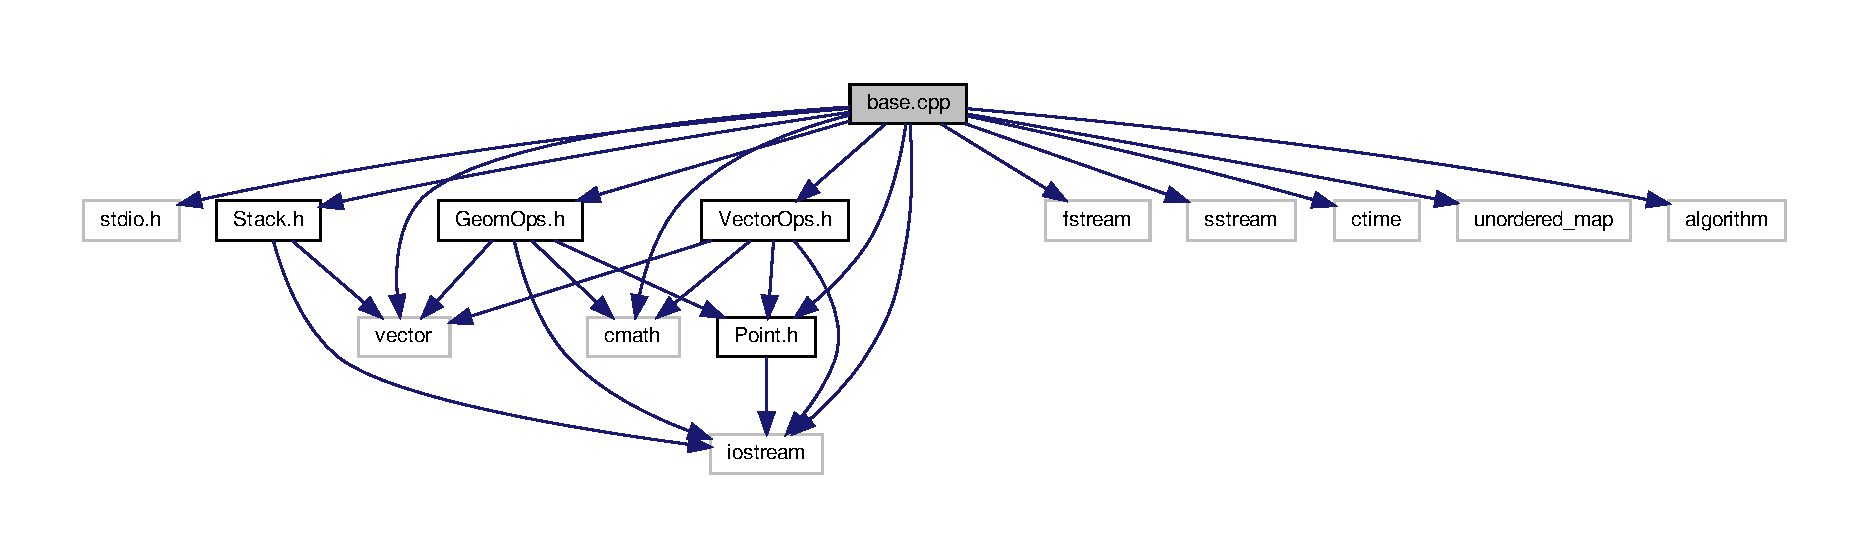
\includegraphics[width=350pt]{base_8cpp__incl}
\end{center}
\end{figure}
\subsection*{Macros}
\begin{DoxyCompactItemize}
\item 
\#define \hyperlink{base_8cpp_a8d58e214b7b5b075466aecc6c0c295ed}{k0}~5
\end{DoxyCompactItemize}
\subsection*{Functions}
\begin{DoxyCompactItemize}
\item 
std\+::vector$<$ \hyperlink{classPoint}{Point} $>$ \hyperlink{base_8cpp_aaf086374b67db32dc76ec43ba7158b0a}{upper\+Hull} (\hyperlink{classPoint}{Point} p\+Min, \hyperlink{classPoint}{Point} p\+Max, std\+::vector$<$ \hyperlink{classPoint}{Point} $>$ points, int num\+\_\+points, int depth)
\item 
std\+::vector$<$ \hyperlink{classPoint}{Point} $>$ \hyperlink{base_8cpp_a716ae214ced649159d3ab9c0aa46c8a6}{lower\+Hull} (\hyperlink{classPoint}{Point} p\+Min, \hyperlink{classPoint}{Point} p\+Max, std\+::vector$<$ \hyperlink{classPoint}{Point} $>$ points, int num\+\_\+points, int depth)
\item 
bool \hyperlink{base_8cpp_a12eda38a151ca94e4b50b21d0d6ae028}{comparator} (\hyperlink{classPoint}{Point} p1, \hyperlink{classPoint}{Point} p2)
\item 
vector$<$ \hyperlink{classPoint}{Point} $>$ \hyperlink{base_8cpp_a40da521b25e7c5fc8c40f1362695a64a}{graham\+Scan} (vector$<$ \hyperlink{classPoint}{Point} $>$ points, int num\+\_\+points)
\item 
void \hyperlink{base_8cpp_a7f49339c6980bcdff628dc6a44456c34}{jarvis\+March} (vector$<$ int $>$ \&hull, vector$<$ \hyperlink{classPoint}{Point} $>$ points, int num\+\_\+points)
\item 
vector$<$ \hyperlink{classPoint}{Point} $>$ \hyperlink{base_8cpp_a322f277b070fa996aa7f5188b37d9937}{k\+PS} (vector$<$ \hyperlink{classPoint}{Point} $>$ points, int num\+\_\+points)
\item 
pair$<$ \hyperlink{classPoint}{Point}, \hyperlink{classPoint}{Point} $>$ \hyperlink{base_8cpp_aa2c1ef29af92ec11da3690a09f503704}{upper\+Bridge} (std\+::vector$<$ \hyperlink{classPoint}{Point} $>$ S, int num\+\_\+points, \hyperlink{classPoint}{Point} L, int depth)
\item 
pair$<$ \hyperlink{classPoint}{Point}, \hyperlink{classPoint}{Point} $>$ \hyperlink{base_8cpp_a4a7415faa1cd0bc5e7cf0dca52bd784d}{lower\+Bridge} (std\+::vector$<$ \hyperlink{classPoint}{Point} $>$ S, int num\+\_\+points, \hyperlink{classPoint}{Point} L, int depth)
\item 
int \hyperlink{base_8cpp_a3c04138a5bfe5d72780bb7e82a18e627}{main} (int argc, char $\ast$$\ast$argv)
\end{DoxyCompactItemize}
\subsection*{Variables}
\begin{DoxyCompactItemize}
\item 
\hyperlink{classGeomOps}{Geom\+Ops} \hyperlink{base_8cpp_aff7f7c491b6084f51cbd483d49675da4}{geom\+A\+PI}
\begin{DoxyCompactList}\small\item\em Provides all the geometrical operations useful for various convex hull methods (imported file) \end{DoxyCompactList}\item 
\hyperlink{classVectorOps}{Vector\+Ops} \hyperlink{base_8cpp_aa9702cb712e0ee9d47c426c78a40f8f7}{vec\+A\+PI}
\begin{DoxyCompactList}\small\item\em Provides all the median algorithms required for convex hull algorithms. \end{DoxyCompactList}\end{DoxyCompactItemize}


\subsection{Macro Definition Documentation}
\mbox{\Hypertarget{base_8cpp_a8d58e214b7b5b075466aecc6c0c295ed}\label{base_8cpp_a8d58e214b7b5b075466aecc6c0c295ed}} 
\index{base.\+cpp@{base.\+cpp}!k0@{k0}}
\index{k0@{k0}!base.\+cpp@{base.\+cpp}}
\subsubsection{\texorpdfstring{k0}{k0}}
{\footnotesize\ttfamily \#define k0~5}



\subsection{Function Documentation}
\mbox{\Hypertarget{base_8cpp_a12eda38a151ca94e4b50b21d0d6ae028}\label{base_8cpp_a12eda38a151ca94e4b50b21d0d6ae028}} 
\index{base.\+cpp@{base.\+cpp}!comparator@{comparator}}
\index{comparator@{comparator}!base.\+cpp@{base.\+cpp}}
\subsubsection{\texorpdfstring{comparator()}{comparator()}}
{\footnotesize\ttfamily bool comparator (\begin{DoxyParamCaption}\item[{\hyperlink{classPoint}{Point}}]{p1,  }\item[{\hyperlink{classPoint}{Point}}]{p2 }\end{DoxyParamCaption})}

This function helps in comparing signed area of two points w.\+r.\+t reference base point \mbox{\Hypertarget{base_8cpp_a40da521b25e7c5fc8c40f1362695a64a}\label{base_8cpp_a40da521b25e7c5fc8c40f1362695a64a}} 
\index{base.\+cpp@{base.\+cpp}!graham\+Scan@{graham\+Scan}}
\index{graham\+Scan@{graham\+Scan}!base.\+cpp@{base.\+cpp}}
\subsubsection{\texorpdfstring{graham\+Scan()}{grahamScan()}}
{\footnotesize\ttfamily vector$<$\hyperlink{classPoint}{Point}$>$ graham\+Scan (\begin{DoxyParamCaption}\item[{vector$<$ \hyperlink{classPoint}{Point} $>$}]{points,  }\item[{int}]{num\+\_\+points }\end{DoxyParamCaption})}

This function gives the points on convec hull for the input set using Graham Scan algorithm 
\begin{DoxyParams}{Parameters}
{\em points} & input set of points \\
\hline
{\em num\+\_\+points} & number of points in input \\
\hline
\end{DoxyParams}
\begin{DoxyReturn}{Returns}
return points on the convex hull 
\end{DoxyReturn}
\mbox{\Hypertarget{base_8cpp_a7f49339c6980bcdff628dc6a44456c34}\label{base_8cpp_a7f49339c6980bcdff628dc6a44456c34}} 
\index{base.\+cpp@{base.\+cpp}!jarvis\+March@{jarvis\+March}}
\index{jarvis\+March@{jarvis\+March}!base.\+cpp@{base.\+cpp}}
\subsubsection{\texorpdfstring{jarvis\+March()}{jarvisMarch()}}
{\footnotesize\ttfamily void jarvis\+March (\begin{DoxyParamCaption}\item[{vector$<$ int $>$ \&}]{hull,  }\item[{vector$<$ \hyperlink{classPoint}{Point} $>$}]{points,  }\item[{int}]{num\+\_\+points }\end{DoxyParamCaption})}

This function gives convex hull for a set of points using Jarvis March Algorithm 
\begin{DoxyParams}{Parameters}
{\em hull} & This is the hull vector to be filled using the algorithm \\
\hline
{\em points} & This is the set of input points \\
\hline
{\em num\+\_\+points} & Number of points in input \\
\hline
\end{DoxyParams}
\mbox{\Hypertarget{base_8cpp_a322f277b070fa996aa7f5188b37d9937}\label{base_8cpp_a322f277b070fa996aa7f5188b37d9937}} 
\index{base.\+cpp@{base.\+cpp}!k\+PS@{k\+PS}}
\index{k\+PS@{k\+PS}!base.\+cpp@{base.\+cpp}}
\subsubsection{\texorpdfstring{k\+P\+S()}{kPS()}}
{\footnotesize\ttfamily vector$<$\hyperlink{classPoint}{Point}$>$ k\+PS (\begin{DoxyParamCaption}\item[{vector$<$ \hyperlink{classPoint}{Point} $>$}]{points,  }\item[{int}]{num\+\_\+points }\end{DoxyParamCaption})}

This function gives convex hull for a set of points using Kirkpatrick Siedel Algorithm 
\begin{DoxyParams}{Parameters}
{\em points} & Set of input points \\
\hline
{\em number} & of points in input \\
\hline
\end{DoxyParams}
\begin{DoxyReturn}{Returns}
set of points in hull 
\end{DoxyReturn}
\mbox{\Hypertarget{base_8cpp_a4a7415faa1cd0bc5e7cf0dca52bd784d}\label{base_8cpp_a4a7415faa1cd0bc5e7cf0dca52bd784d}} 
\index{base.\+cpp@{base.\+cpp}!lower\+Bridge@{lower\+Bridge}}
\index{lower\+Bridge@{lower\+Bridge}!base.\+cpp@{base.\+cpp}}
\subsubsection{\texorpdfstring{lower\+Bridge()}{lowerBridge()}}
{\footnotesize\ttfamily pair$<$\hyperlink{classPoint}{Point},\hyperlink{classPoint}{Point}$>$ lower\+Bridge (\begin{DoxyParamCaption}\item[{std\+::vector$<$ \hyperlink{classPoint}{Point} $>$}]{S,  }\item[{int}]{num\+\_\+points,  }\item[{\hyperlink{classPoint}{Point}}]{L,  }\item[{int}]{depth }\end{DoxyParamCaption})}

This function finds of lower bridge line described by the two points 
\begin{DoxyParams}{Parameters}
{\em S} & input set of points \\
\hline
{\em num\+\_\+points} & number of points in input \\
\hline
{\em L} & median line described by a point \\
\hline
{\em depth} & number of times the function has recursed \\
\hline
\end{DoxyParams}
\begin{DoxyReturn}{Returns}
returns a pair of points describing lower bridge 
\end{DoxyReturn}
\mbox{\Hypertarget{base_8cpp_a716ae214ced649159d3ab9c0aa46c8a6}\label{base_8cpp_a716ae214ced649159d3ab9c0aa46c8a6}} 
\index{base.\+cpp@{base.\+cpp}!lower\+Hull@{lower\+Hull}}
\index{lower\+Hull@{lower\+Hull}!base.\+cpp@{base.\+cpp}}
\subsubsection{\texorpdfstring{lower\+Hull()}{lowerHull()}}
{\footnotesize\ttfamily std\+::vector$<$ \hyperlink{classPoint}{Point} $>$ lower\+Hull (\begin{DoxyParamCaption}\item[{\hyperlink{classPoint}{Point}}]{p\+Min,  }\item[{\hyperlink{classPoint}{Point}}]{p\+Max,  }\item[{std\+::vector$<$ \hyperlink{classPoint}{Point} $>$}]{points,  }\item[{int}]{num\+\_\+points,  }\item[{int}]{depth }\end{DoxyParamCaption})}

This function calculates lower hull from given set of points 
\begin{DoxyParams}{Parameters}
{\em p\+Min} & \hyperlink{classPoint}{Point} with minimum x coordinate \\
\hline
{\em p\+Max} & \hyperlink{classPoint}{Point} with maximum x coordinate \\
\hline
{\em points} & set of input points \\
\hline
{\em num\+\_\+points} & number of points in input \\
\hline
{\em depth} & number of times the function is recursed \\
\hline
\end{DoxyParams}
\begin{DoxyReturn}{Returns}
Returns a set of points in lower hull 
\end{DoxyReturn}
\mbox{\Hypertarget{base_8cpp_a3c04138a5bfe5d72780bb7e82a18e627}\label{base_8cpp_a3c04138a5bfe5d72780bb7e82a18e627}} 
\index{base.\+cpp@{base.\+cpp}!main@{main}}
\index{main@{main}!base.\+cpp@{base.\+cpp}}
\subsubsection{\texorpdfstring{main()}{main()}}
{\footnotesize\ttfamily int main (\begin{DoxyParamCaption}\item[{int}]{argc,  }\item[{char $\ast$$\ast$}]{argv }\end{DoxyParamCaption})}

\mbox{\Hypertarget{base_8cpp_aa2c1ef29af92ec11da3690a09f503704}\label{base_8cpp_aa2c1ef29af92ec11da3690a09f503704}} 
\index{base.\+cpp@{base.\+cpp}!upper\+Bridge@{upper\+Bridge}}
\index{upper\+Bridge@{upper\+Bridge}!base.\+cpp@{base.\+cpp}}
\subsubsection{\texorpdfstring{upper\+Bridge()}{upperBridge()}}
{\footnotesize\ttfamily pair$<$\hyperlink{classPoint}{Point},\hyperlink{classPoint}{Point}$>$ upper\+Bridge (\begin{DoxyParamCaption}\item[{std\+::vector$<$ \hyperlink{classPoint}{Point} $>$}]{S,  }\item[{int}]{num\+\_\+points,  }\item[{\hyperlink{classPoint}{Point}}]{L,  }\item[{int}]{depth }\end{DoxyParamCaption})}

This function finds of upper bridge line described by the two points 
\begin{DoxyParams}{Parameters}
{\em S} & input set of points \\
\hline
{\em num\+\_\+points} & number of points in input \\
\hline
{\em L} & median line described by a point \\
\hline
{\em depth} & number of times the function has recursed \\
\hline
\end{DoxyParams}
\begin{DoxyReturn}{Returns}
returns a pair of points describing upper bridge 
\end{DoxyReturn}
\mbox{\Hypertarget{base_8cpp_aaf086374b67db32dc76ec43ba7158b0a}\label{base_8cpp_aaf086374b67db32dc76ec43ba7158b0a}} 
\index{base.\+cpp@{base.\+cpp}!upper\+Hull@{upper\+Hull}}
\index{upper\+Hull@{upper\+Hull}!base.\+cpp@{base.\+cpp}}
\subsubsection{\texorpdfstring{upper\+Hull()}{upperHull()}}
{\footnotesize\ttfamily std\+::vector$<$ \hyperlink{classPoint}{Point} $>$ upper\+Hull (\begin{DoxyParamCaption}\item[{\hyperlink{classPoint}{Point}}]{p\+Min,  }\item[{\hyperlink{classPoint}{Point}}]{p\+Max,  }\item[{std\+::vector$<$ \hyperlink{classPoint}{Point} $>$}]{points,  }\item[{int}]{num\+\_\+points,  }\item[{int}]{depth }\end{DoxyParamCaption})}

This function calculates upper hull from given set of points 
\begin{DoxyParams}{Parameters}
{\em p\+Min} & \hyperlink{classPoint}{Point} with minimum x coordinate \\
\hline
{\em p\+Max} & \hyperlink{classPoint}{Point} with maximum x coordinate \\
\hline
{\em points} & set of input points \\
\hline
{\em num\+\_\+points} & number of points in input \\
\hline
{\em depth} & number of times the function is recursed \\
\hline
\end{DoxyParams}
\begin{DoxyReturn}{Returns}
Returns a set of points in upper hull 
\end{DoxyReturn}


\subsection{Variable Documentation}
\mbox{\Hypertarget{base_8cpp_aff7f7c491b6084f51cbd483d49675da4}\label{base_8cpp_aff7f7c491b6084f51cbd483d49675da4}} 
\index{base.\+cpp@{base.\+cpp}!geom\+A\+PI@{geom\+A\+PI}}
\index{geom\+A\+PI@{geom\+A\+PI}!base.\+cpp@{base.\+cpp}}
\subsubsection{\texorpdfstring{geom\+A\+PI}{geomAPI}}
{\footnotesize\ttfamily \hyperlink{classGeomOps}{Geom\+Ops} geom\+A\+PI}



Provides all the geometrical operations useful for various convex hull methods (imported file) 

\mbox{\Hypertarget{base_8cpp_aa9702cb712e0ee9d47c426c78a40f8f7}\label{base_8cpp_aa9702cb712e0ee9d47c426c78a40f8f7}} 
\index{base.\+cpp@{base.\+cpp}!vec\+A\+PI@{vec\+A\+PI}}
\index{vec\+A\+PI@{vec\+A\+PI}!base.\+cpp@{base.\+cpp}}
\subsubsection{\texorpdfstring{vec\+A\+PI}{vecAPI}}
{\footnotesize\ttfamily \hyperlink{classVectorOps}{Vector\+Ops} vec\+A\+PI}



Provides all the median algorithms required for convex hull algorithms. 


\hypertarget{GeomOps_8cpp}{}\section{Geom\+Ops.\+cpp File Reference}
\label{GeomOps_8cpp}\index{Geom\+Ops.\+cpp@{Geom\+Ops.\+cpp}}
{\ttfamily \#include $<$iostream$>$}\newline
{\ttfamily \#include $<$vector$>$}\newline
{\ttfamily \#include $<$cmath$>$}\newline
{\ttfamily \#include \char`\"{}Point.\+h\char`\"{}}\newline
{\ttfamily \#include \char`\"{}Geom\+Ops.\+h\char`\"{}}\newline
Include dependency graph for Geom\+Ops.\+cpp\+:
\nopagebreak
\begin{figure}[H]
\begin{center}
\leavevmode
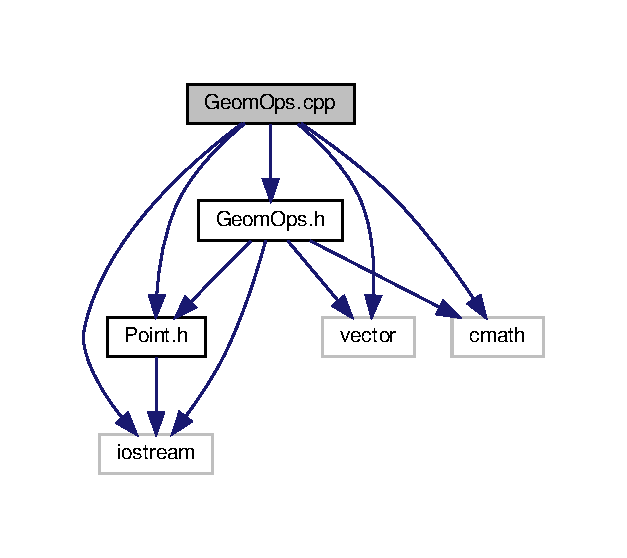
\includegraphics[width=301pt]{GeomOps_8cpp__incl}
\end{center}
\end{figure}

\hypertarget{GeomOps_8h}{}\section{Geom\+Ops.\+h File Reference}
\label{GeomOps_8h}\index{Geom\+Ops.\+h@{Geom\+Ops.\+h}}
{\ttfamily \#include $<$iostream$>$}\newline
{\ttfamily \#include $<$vector$>$}\newline
{\ttfamily \#include $<$cmath$>$}\newline
{\ttfamily \#include \char`\"{}Point.\+h\char`\"{}}\newline
Include dependency graph for Geom\+Ops.\+h\+:
\nopagebreak
\begin{figure}[H]
\begin{center}
\leavevmode
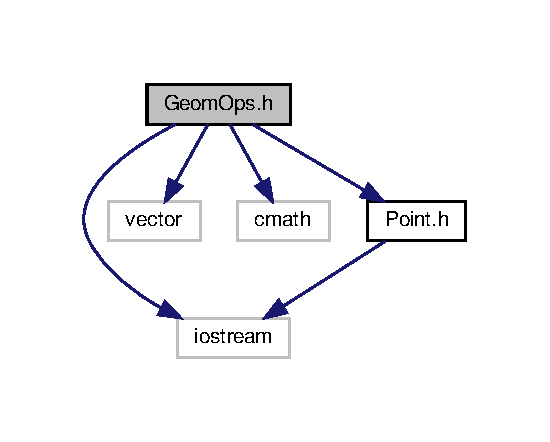
\includegraphics[width=264pt]{GeomOps_8h__incl}
\end{center}
\end{figure}
This graph shows which files directly or indirectly include this file\+:
\nopagebreak
\begin{figure}[H]
\begin{center}
\leavevmode
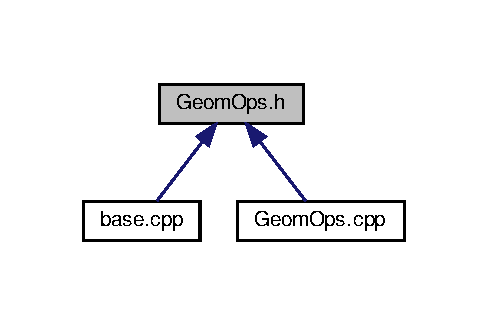
\includegraphics[width=234pt]{GeomOps_8h__dep__incl}
\end{center}
\end{figure}
\subsection*{Classes}
\begin{DoxyCompactItemize}
\item 
class \hyperlink{classGeomOps}{Geom\+Ops}
\end{DoxyCompactItemize}

\hypertarget{plotJM_8py}{}\section{plot\+J\+M.\+py File Reference}
\label{plotJM_8py}\index{plot\+J\+M.\+py@{plot\+J\+M.\+py}}
\subsection*{Namespaces}
\begin{DoxyCompactItemize}
\item 
 \hyperlink{namespaceplotJM}{plot\+JM}
\end{DoxyCompactItemize}
\subsection*{Variables}
\begin{DoxyCompactItemize}
\item 
int \hyperlink{namespaceplotJM_aa893f2c8f47574915a4cc130164ba160}{plot\+J\+M.\+num} = 1
\item 
string \hyperlink{namespaceplotJM_aece5bd26b7eba5b9cc746654691880c0}{plot\+J\+M.\+type} = \char`\"{}JM\char`\"{}
\item 
string \hyperlink{namespaceplotJM_a7e306c9d020e3a82daec94c8a7981b5e}{plot\+J\+M.\+path\+Points} = os.\+getcwd()+\textquotesingle{}/input/input\textquotesingle{}+str(num)+\textquotesingle{}.txt\textquotesingle{}
\item 
string \hyperlink{namespaceplotJM_acd0ae8ec083c4b2359bb23875bb4792c}{plot\+J\+M.\+path\+Indices} = os.\+getcwd()+\textquotesingle{}/output\+JM/output\textquotesingle{}+str(num)+type+\textquotesingle{}.txt\textquotesingle{}
\item 
list \hyperlink{namespaceplotJM_a4736c91f6642a68255bc59e25177f6b6}{plot\+J\+M.\+points} = \mbox{[}$\,$\mbox{]}
\item 
\hyperlink{namespaceplotJM_a1981504f48dad7742cddc6613eb4819f}{plot\+J\+M.\+points\+File} = open(path\+Points,\textquotesingle{}r\textquotesingle{})
\item 
list \hyperlink{namespaceplotJM_ac8a0cf53bb644724563a7855b2f1298f}{plot\+J\+M.\+indices} = \mbox{[}$\,$\mbox{]}
\item 
\hyperlink{namespaceplotJM_a5d87970cd85b2ed2de29d310a2c11739}{plot\+J\+M.\+lines\+File} = open(path\+Indices,\textquotesingle{}r\textquotesingle{})
\item 
list \hyperlink{namespaceplotJM_adf22560b07746c190ca82c2067a72af5}{plot\+J\+M.\+pointsX} = \mbox{[}$\,$\mbox{]}
\item 
list \hyperlink{namespaceplotJM_af0fe4115db67f777b24566dca7ae1d83}{plot\+J\+M.\+pointsY} = \mbox{[}$\,$\mbox{]}
\item 
list \hyperlink{namespaceplotJM_a6269675659677b5b402dd2e97fb3d9f6}{plot\+J\+M.\+points\+X\+Full} = \mbox{[}$\,$\mbox{]}
\item 
list \hyperlink{namespaceplotJM_a94cf66896dacc6cbe356a810745e72ff}{plot\+J\+M.\+points\+Y\+Full} = \mbox{[}$\,$\mbox{]}
\item 
\hyperlink{namespaceplotJM_a3eca2b92173774b6200493c52c64dec4}{plot\+J\+M.\+c}
\end{DoxyCompactItemize}

\hypertarget{plotKPS_8py}{}\section{plot\+K\+P\+S.\+py File Reference}
\label{plotKPS_8py}\index{plot\+K\+P\+S.\+py@{plot\+K\+P\+S.\+py}}
\subsection*{Namespaces}
\begin{DoxyCompactItemize}
\item 
 \hyperlink{namespaceplotKPS}{plot\+K\+PS}
\end{DoxyCompactItemize}
\subsection*{Variables}
\begin{DoxyCompactItemize}
\item 
int \hyperlink{namespaceplotKPS_a7d067860f384d4514b73bb9d364df084}{plot\+K\+P\+S.\+num} = 8
\item 
string \hyperlink{namespaceplotKPS_a6f353d1e228ea6b30f24563026ecb40c}{plot\+K\+P\+S.\+type} = \char`\"{}K\+PS\char`\"{}
\item 
string \hyperlink{namespaceplotKPS_abff4301b2725775317d29ad1956d8cc3}{plot\+K\+P\+S.\+path\+Points\+Full} = os.\+getcwd()+\textquotesingle{}/input/input\textquotesingle{}+str(num)+\textquotesingle{}.txt\textquotesingle{}
\item 
list \hyperlink{namespaceplotKPS_a48ccbb4e710dfebea784f34b91a3b8b7}{plot\+K\+P\+S.\+points} = \mbox{[}$\,$\mbox{]}
\item 
\hyperlink{namespaceplotKPS_a163726d3306fbdcaaa77215db0205452}{plot\+K\+P\+S.\+points\+Full\+File} = open(path\+Points\+Full,\textquotesingle{}r\textquotesingle{})
\item 
list \hyperlink{namespaceplotKPS_aca0b8d5972b4405cee64b721b05fe69b}{plot\+K\+P\+S.\+points\+X\+Full} = \mbox{[}$\,$\mbox{]}
\item 
list \hyperlink{namespaceplotKPS_ad03be08fd881cef42cd8fbb5dda7d68e}{plot\+K\+P\+S.\+points\+Y\+Full} = \mbox{[}$\,$\mbox{]}
\item 
string \hyperlink{namespaceplotKPS_a67510e87215a8d35ba91887dad2ce7c0}{plot\+K\+P\+S.\+path\+Points} = os.\+getcwd()+\textquotesingle{}/output\textquotesingle{}+type+\textquotesingle{}/output\textquotesingle{}+str(num)+type+\textquotesingle{}.txt\textquotesingle{}
\item 
\hyperlink{namespaceplotKPS_ac7f5dbe4ce237b1140497a2bf4fbf16e}{plot\+K\+P\+S.\+points\+File} = open(path\+Points,\textquotesingle{}r\textquotesingle{})
\item 
list \hyperlink{namespaceplotKPS_abd755cad257acc579edd18d4fc485ae6}{plot\+K\+P\+S.\+pointsX} = \mbox{[}$\,$\mbox{]}
\item 
list \hyperlink{namespaceplotKPS_afe7f323931691a3471bbf3f21066f2ec}{plot\+K\+P\+S.\+pointsY} = \mbox{[}$\,$\mbox{]}
\item 
\hyperlink{namespaceplotKPS_ac5170bd98bd37eefaafd02ca9e4afddb}{plot\+K\+P\+S.\+c}
\end{DoxyCompactItemize}

\hypertarget{Point_8cpp}{}\section{Point.\+cpp File Reference}
\label{Point_8cpp}\index{Point.\+cpp@{Point.\+cpp}}
{\ttfamily \#include $<$iostream$>$}\newline
{\ttfamily \#include \char`\"{}Point.\+h\char`\"{}}\newline
Include dependency graph for Point.\+cpp\+:
\nopagebreak
\begin{figure}[H]
\begin{center}
\leavevmode
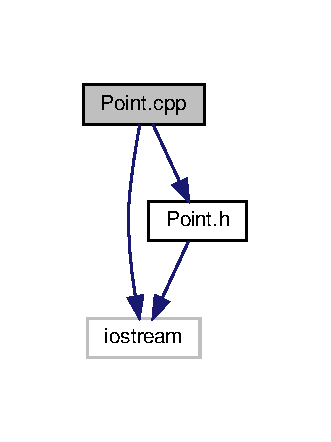
\includegraphics[width=159pt]{Point_8cpp__incl}
\end{center}
\end{figure}

\hypertarget{Point_8h}{}\section{Point.\+h File Reference}
\label{Point_8h}\index{Point.\+h@{Point.\+h}}
{\ttfamily \#include $<$iostream$>$}\newline
Include dependency graph for Point.\+h\+:
\nopagebreak
\begin{figure}[H]
\begin{center}
\leavevmode
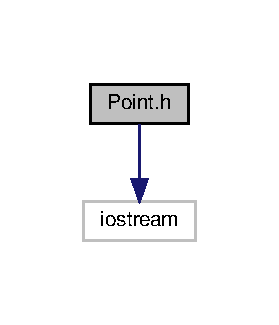
\includegraphics[width=134pt]{Point_8h__incl}
\end{center}
\end{figure}
This graph shows which files directly or indirectly include this file\+:
\nopagebreak
\begin{figure}[H]
\begin{center}
\leavevmode
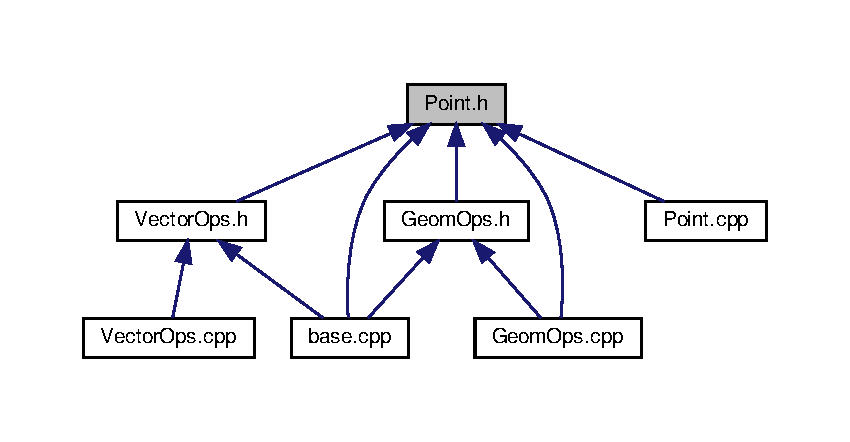
\includegraphics[width=350pt]{Point_8h__dep__incl}
\end{center}
\end{figure}
\subsection*{Classes}
\begin{DoxyCompactItemize}
\item 
class \hyperlink{classPoint}{Point}
\begin{DoxyCompactList}\small\item\em This defines a 2-\/D point with common functionalities to set and retrieve coordinate values. \end{DoxyCompactList}\end{DoxyCompactItemize}

\hypertarget{README_8md}{}\section{R\+E\+A\+D\+M\+E.\+md File Reference}
\label{README_8md}\index{R\+E\+A\+D\+M\+E.\+md@{R\+E\+A\+D\+M\+E.\+md}}

\hypertarget{Stack_8h}{}\section{Stack.\+h File Reference}
\label{Stack_8h}\index{Stack.\+h@{Stack.\+h}}
{\ttfamily \#include $<$iostream$>$}\newline
{\ttfamily \#include $<$vector$>$}\newline
Include dependency graph for Stack.\+h\+:
\nopagebreak
\begin{figure}[H]
\begin{center}
\leavevmode
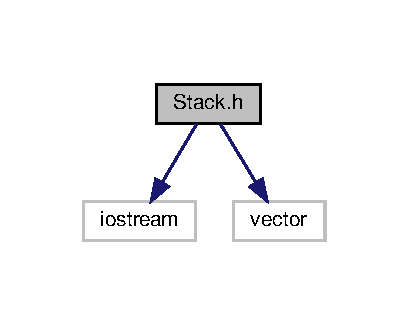
\includegraphics[width=196pt]{Stack_8h__incl}
\end{center}
\end{figure}
This graph shows which files directly or indirectly include this file\+:
\nopagebreak
\begin{figure}[H]
\begin{center}
\leavevmode
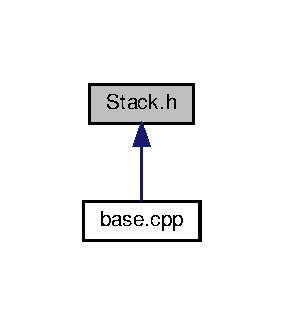
\includegraphics[width=136pt]{Stack_8h__dep__incl}
\end{center}
\end{figure}
\subsection*{Classes}
\begin{DoxyCompactItemize}
\item 
class \hyperlink{classStack}{Stack$<$ T $>$}
\begin{DoxyCompactList}\small\item\em Simple \hyperlink{classStack}{Stack} implementation. \end{DoxyCompactList}\end{DoxyCompactItemize}
\subsection*{Macros}
\begin{DoxyCompactItemize}
\item 
\#define \hyperlink{Stack_8h_a392fb874e547e582e9c66a08a1f23326}{M\+AX}~10000
\end{DoxyCompactItemize}


\subsection{Macro Definition Documentation}
\mbox{\Hypertarget{Stack_8h_a392fb874e547e582e9c66a08a1f23326}\label{Stack_8h_a392fb874e547e582e9c66a08a1f23326}} 
\index{Stack.\+h@{Stack.\+h}!M\+AX@{M\+AX}}
\index{M\+AX@{M\+AX}!Stack.\+h@{Stack.\+h}}
\subsubsection{\texorpdfstring{M\+AX}{MAX}}
{\footnotesize\ttfamily \#define M\+AX~10000}


\hypertarget{VectorOps_8cpp}{}\section{Vector\+Ops.\+cpp File Reference}
\label{VectorOps_8cpp}\index{Vector\+Ops.\+cpp@{Vector\+Ops.\+cpp}}
{\ttfamily \#include $<$iostream$>$}\newline
{\ttfamily \#include $<$vector$>$}\newline
{\ttfamily \#include $<$cmath$>$}\newline
{\ttfamily \#include $<$algorithm$>$}\newline
{\ttfamily \#include \char`\"{}Vector\+Ops.\+h\char`\"{}}\newline
Include dependency graph for Vector\+Ops.\+cpp\+:
\nopagebreak
\begin{figure}[H]
\begin{center}
\leavevmode
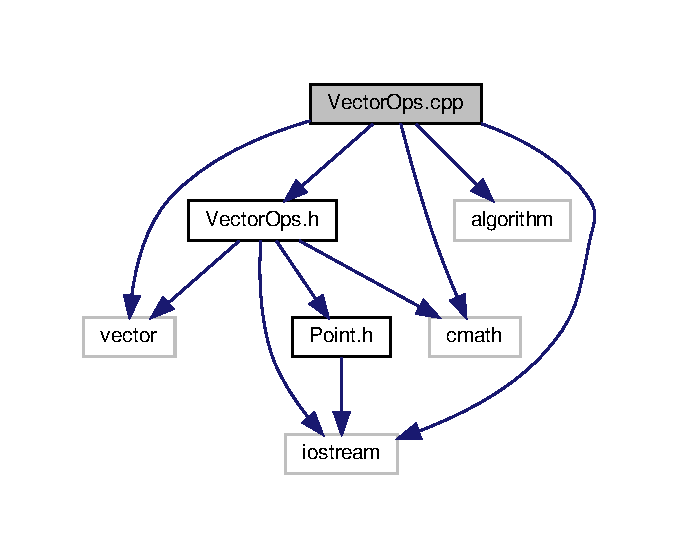
\includegraphics[width=326pt]{VectorOps_8cpp__incl}
\end{center}
\end{figure}

\hypertarget{VectorOps_8h}{}\section{Vector\+Ops.\+h File Reference}
\label{VectorOps_8h}\index{Vector\+Ops.\+h@{Vector\+Ops.\+h}}
{\ttfamily \#include $<$iostream$>$}\newline
{\ttfamily \#include $<$vector$>$}\newline
{\ttfamily \#include $<$cmath$>$}\newline
{\ttfamily \#include \char`\"{}Point.\+h\char`\"{}}\newline
Include dependency graph for Vector\+Ops.\+h\+:
\nopagebreak
\begin{figure}[H]
\begin{center}
\leavevmode
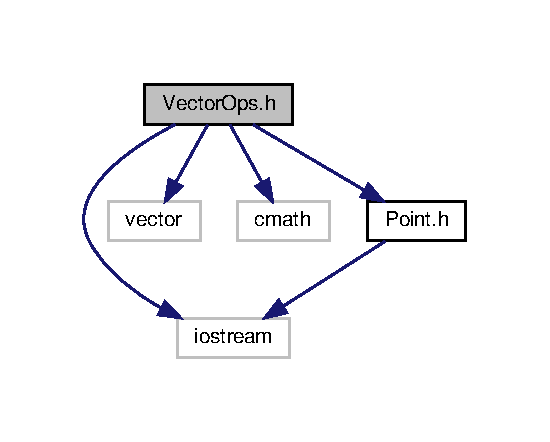
\includegraphics[width=264pt]{VectorOps_8h__incl}
\end{center}
\end{figure}
This graph shows which files directly or indirectly include this file\+:
\nopagebreak
\begin{figure}[H]
\begin{center}
\leavevmode
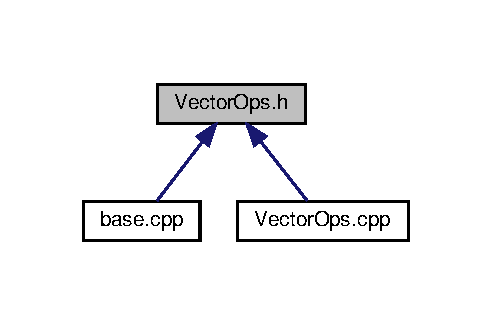
\includegraphics[width=236pt]{VectorOps_8h__dep__incl}
\end{center}
\end{figure}
\subsection*{Classes}
\begin{DoxyCompactItemize}
\item 
class \hyperlink{classVectorOps}{Vector\+Ops}
\end{DoxyCompactItemize}

%--- End generated contents ---

% Index
\backmatter
\newpage
\phantomsection
\clearemptydoublepage
\addcontentsline{toc}{chapter}{Index}
\printindex

\end{document}
